%!TEX root = ../my_thesis.tex
\section{Opposite-side tagging studies}
\label{app:OS}

\subsection[Mass fit of $\Bp\to\Dzb\pip$]{Mass fit of \boldmath{$\Bp\to\Dzb\pip$}}
\label{app:OSmassFit}

A fit to the mass distribution of $\Bp$ candidates is done to calculate \emph{sWeights},
used in the subsequent steps of the analysis to subtract the backgrounds surviving the selection.
A two-step procedure similar to that adopted for the $\Bz\to\Dmp\pipm$ analysis (``Fit A'' in a
wide mass window to account for all backgrounds, and ``Fit B'' in a subset to calculate the weights,
as described in Sec.~\ref{sec:massfit}, where the same mass windows are adopted) is used for the fit of the $\Bp\to\Dzb\pip$ candidates.
The projection of the total PDF on the $\pi$ sample and the $K$ sample (``Fit A'') is shown in
Fig.~\ref{fig:OSmassFit}, as well as the projection of the total PDF in the reduced mass interval (``Fit B'').
The $\pi$ sample and $K$ sample are defined by the PID requirement
on the companion track, PIDK$<5$ and PIDK$>5$, respectively.

The background components expected in the $\pi$ sample for the $\Bp\to\Dzb\pip$ mass fit are listed below,
together with the PDF used for each component:
\begin{itemize}[noitemsep,topsep=0pt]
  \item $\Bp\to\Dzb\pip$: double-sided Hypatia function.
  \item $\Bp\to\Dzb\Kp$: double-sided Hypatia function.
  \item $\Bz\to\Dzb\pip\pim$: Crystal ball function plus Gaussian function.
  \item $\Bp\to\bar D^{0*}\pip$: Johnson SU function plus Gaussian function.
  \item Combinatorial background: single exponential function.  
\end{itemize}
The list of components expected in the $K$ sample is the following:
\begin{itemize}[noitemsep,topsep=0pt]
  \item $\Bp\to\Dzb\pip$: double-sided Hypatia function.
  \item $\Bp\to\Dzb\Kp$: single-sided Hypatia function.
  \item $\Bp\to\bar D^{0*}\pip$: Crystal ball function plus exponential function.
  \item $\Bp\to\Dzb K^{+*}$: Gaussian function.
  \item Combinatorial background: single exponential function.  
\end{itemize}
All the PDFs listed above are defined in Appendix~\ref{app:pdfsdef}. 

The values for the fitted parameters floated in the fit are reported in Table~\ref{tab:OSmassFitA} for Fit A and Table~\ref{tab:OSmassFitB} for Fit B. The naming convention for each parameter is similar to the one used in Sec.~\ref{sec:DataMassFit}.

\begin{figure}[t]
	\begin{center}
		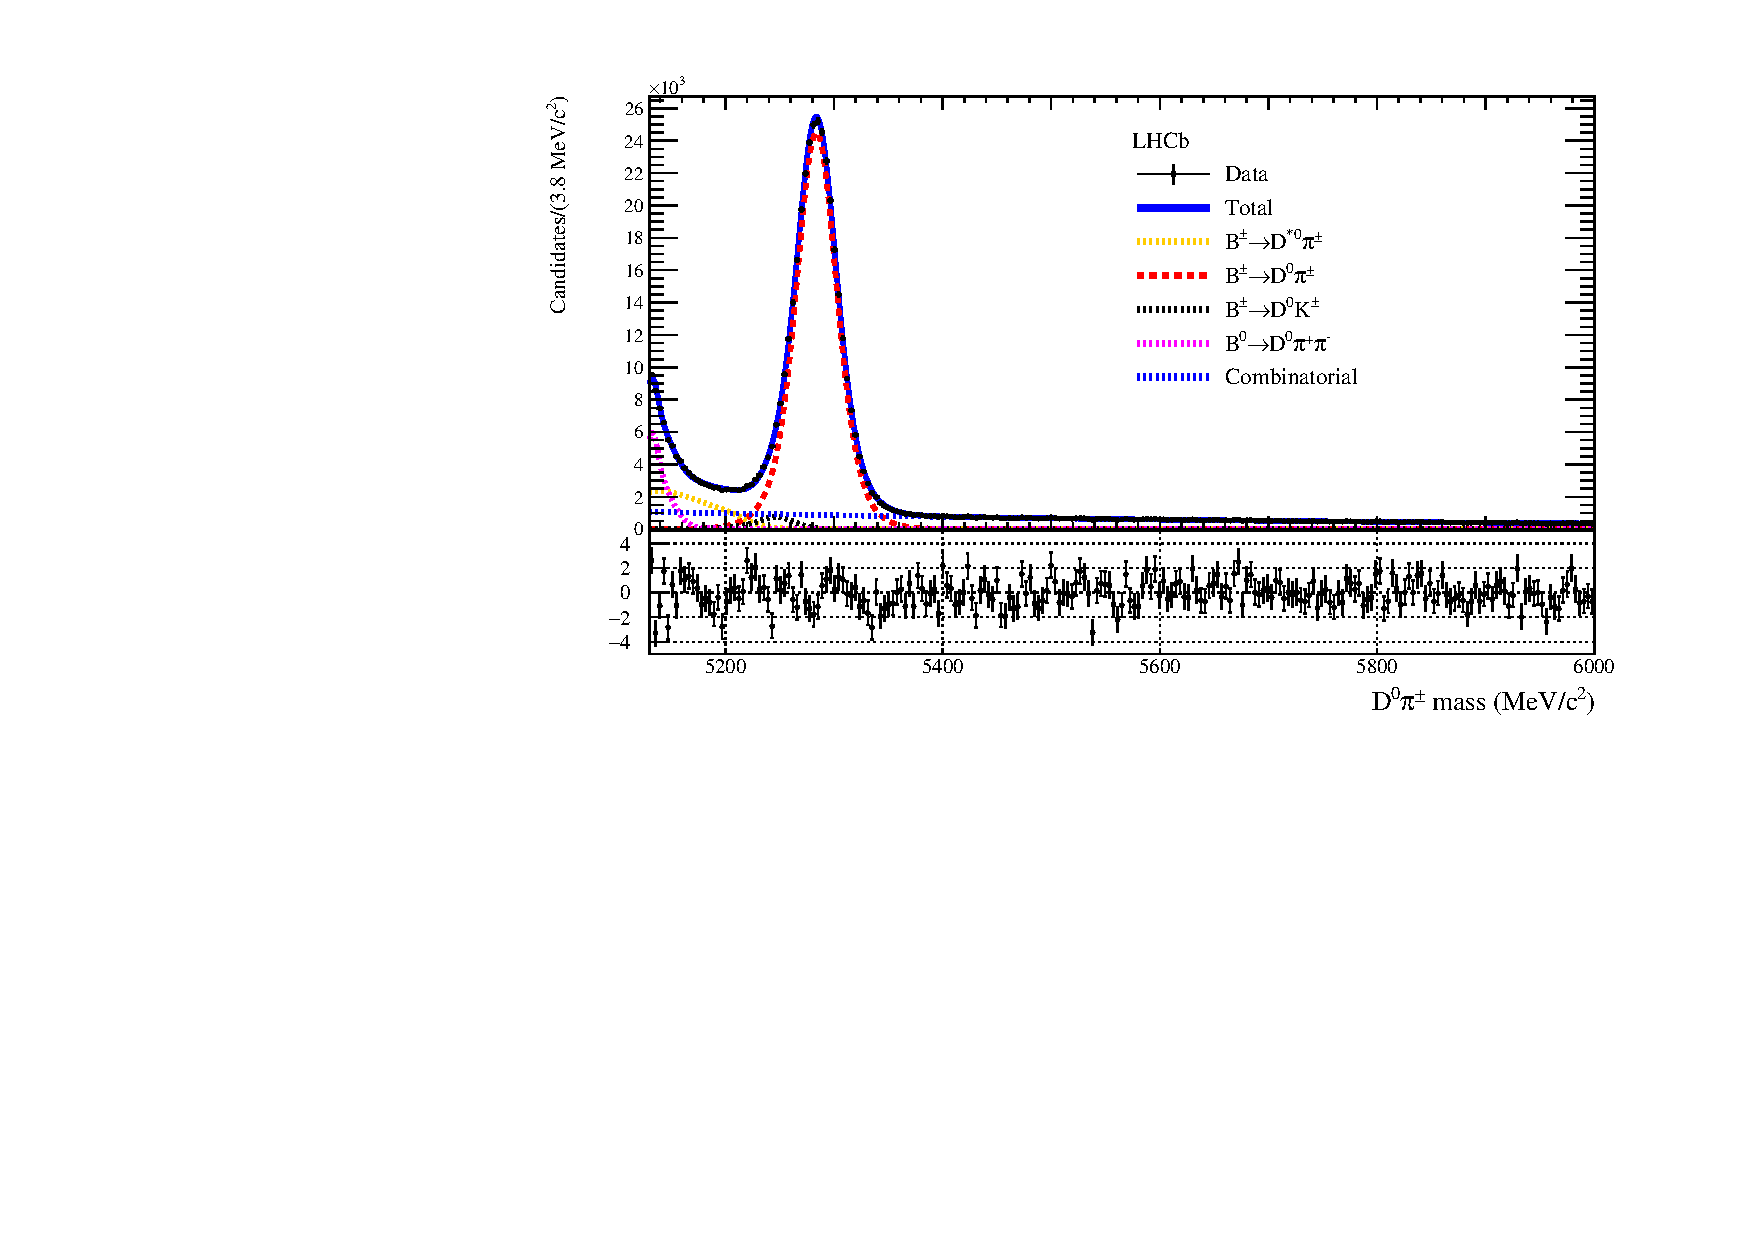
\includegraphics[width=0.49\textwidth]{AA-Appdx-OSTaggers/figs/MDFit_BeautyMass_Bu2D0Pi_withPulls.pdf}
		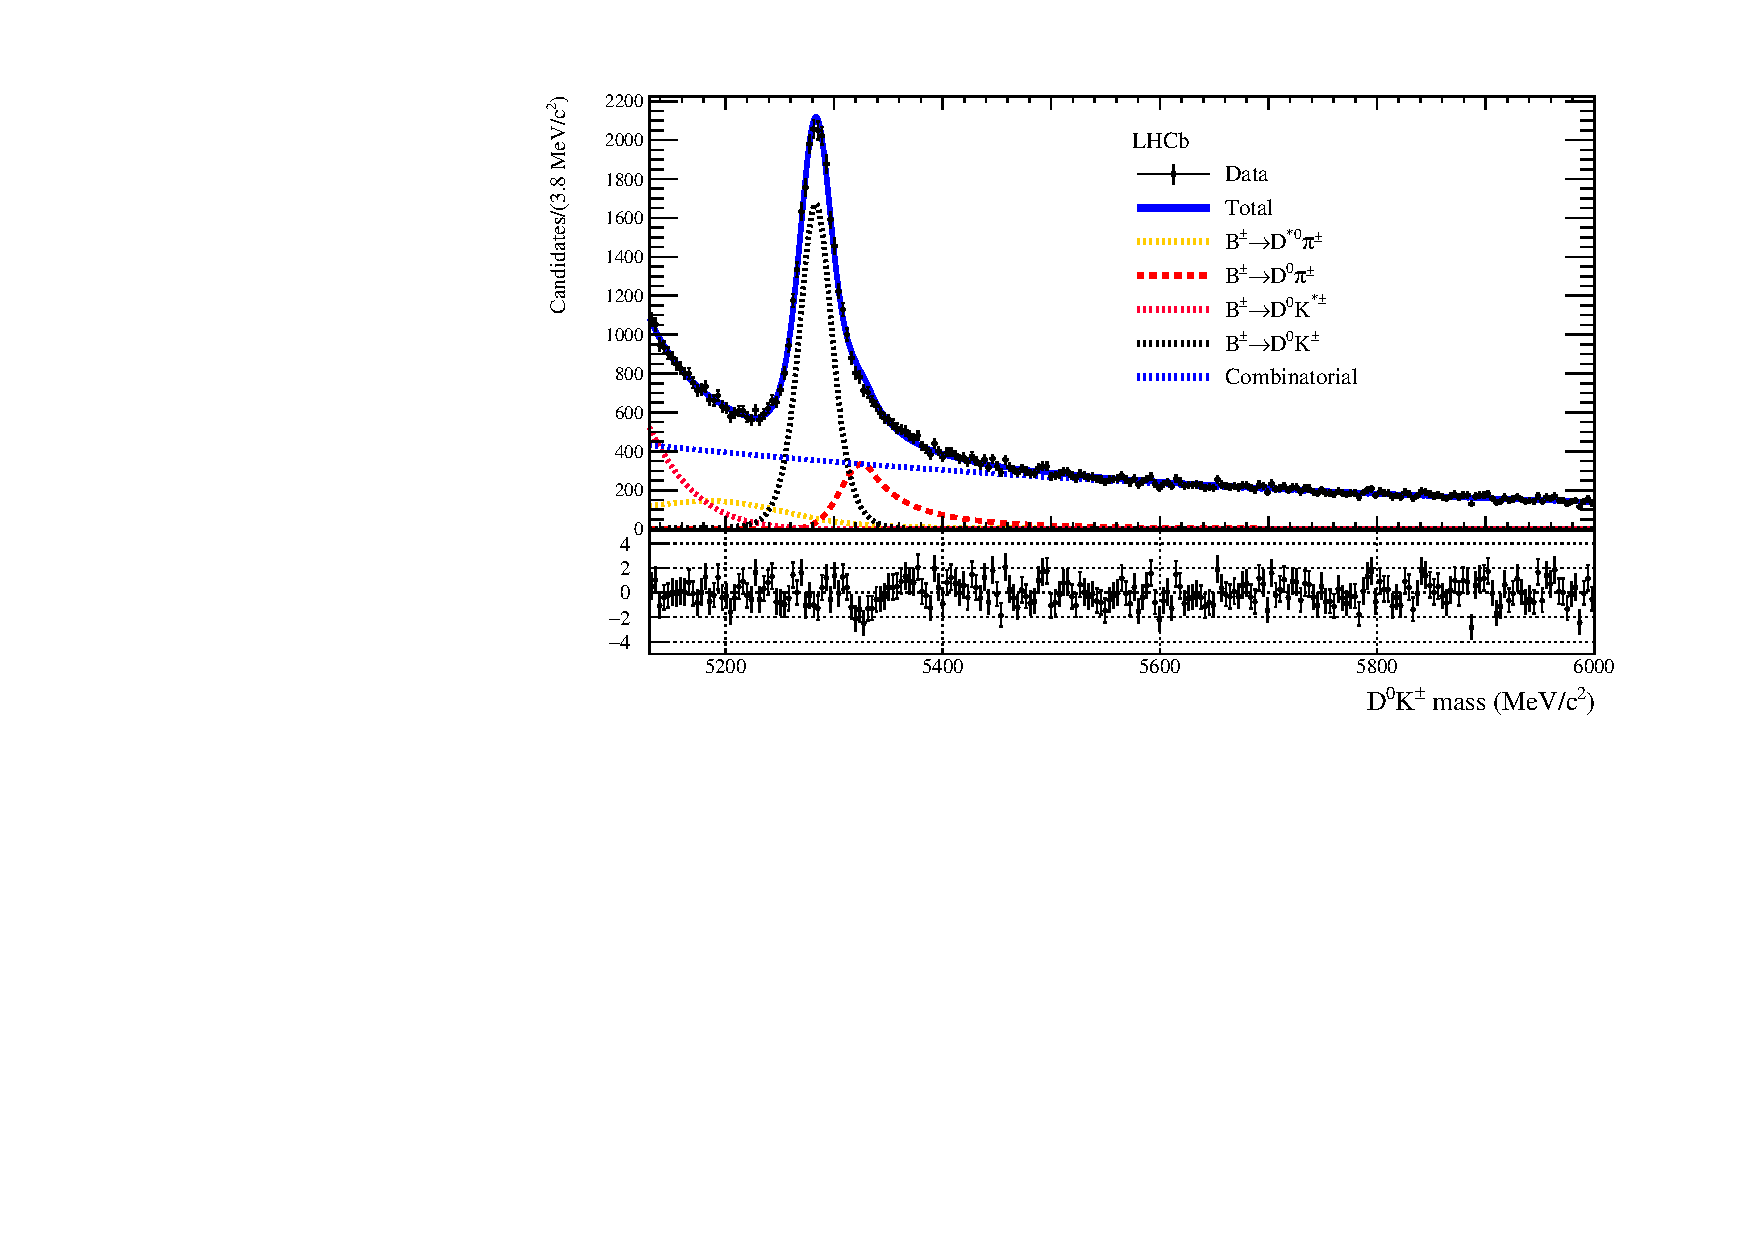
\includegraphics[width=0.49\textwidth]{AA-Appdx-OSTaggers/figs/MDFit_BeautyMass_Bu2D0K_withPulls.pdf} \\
		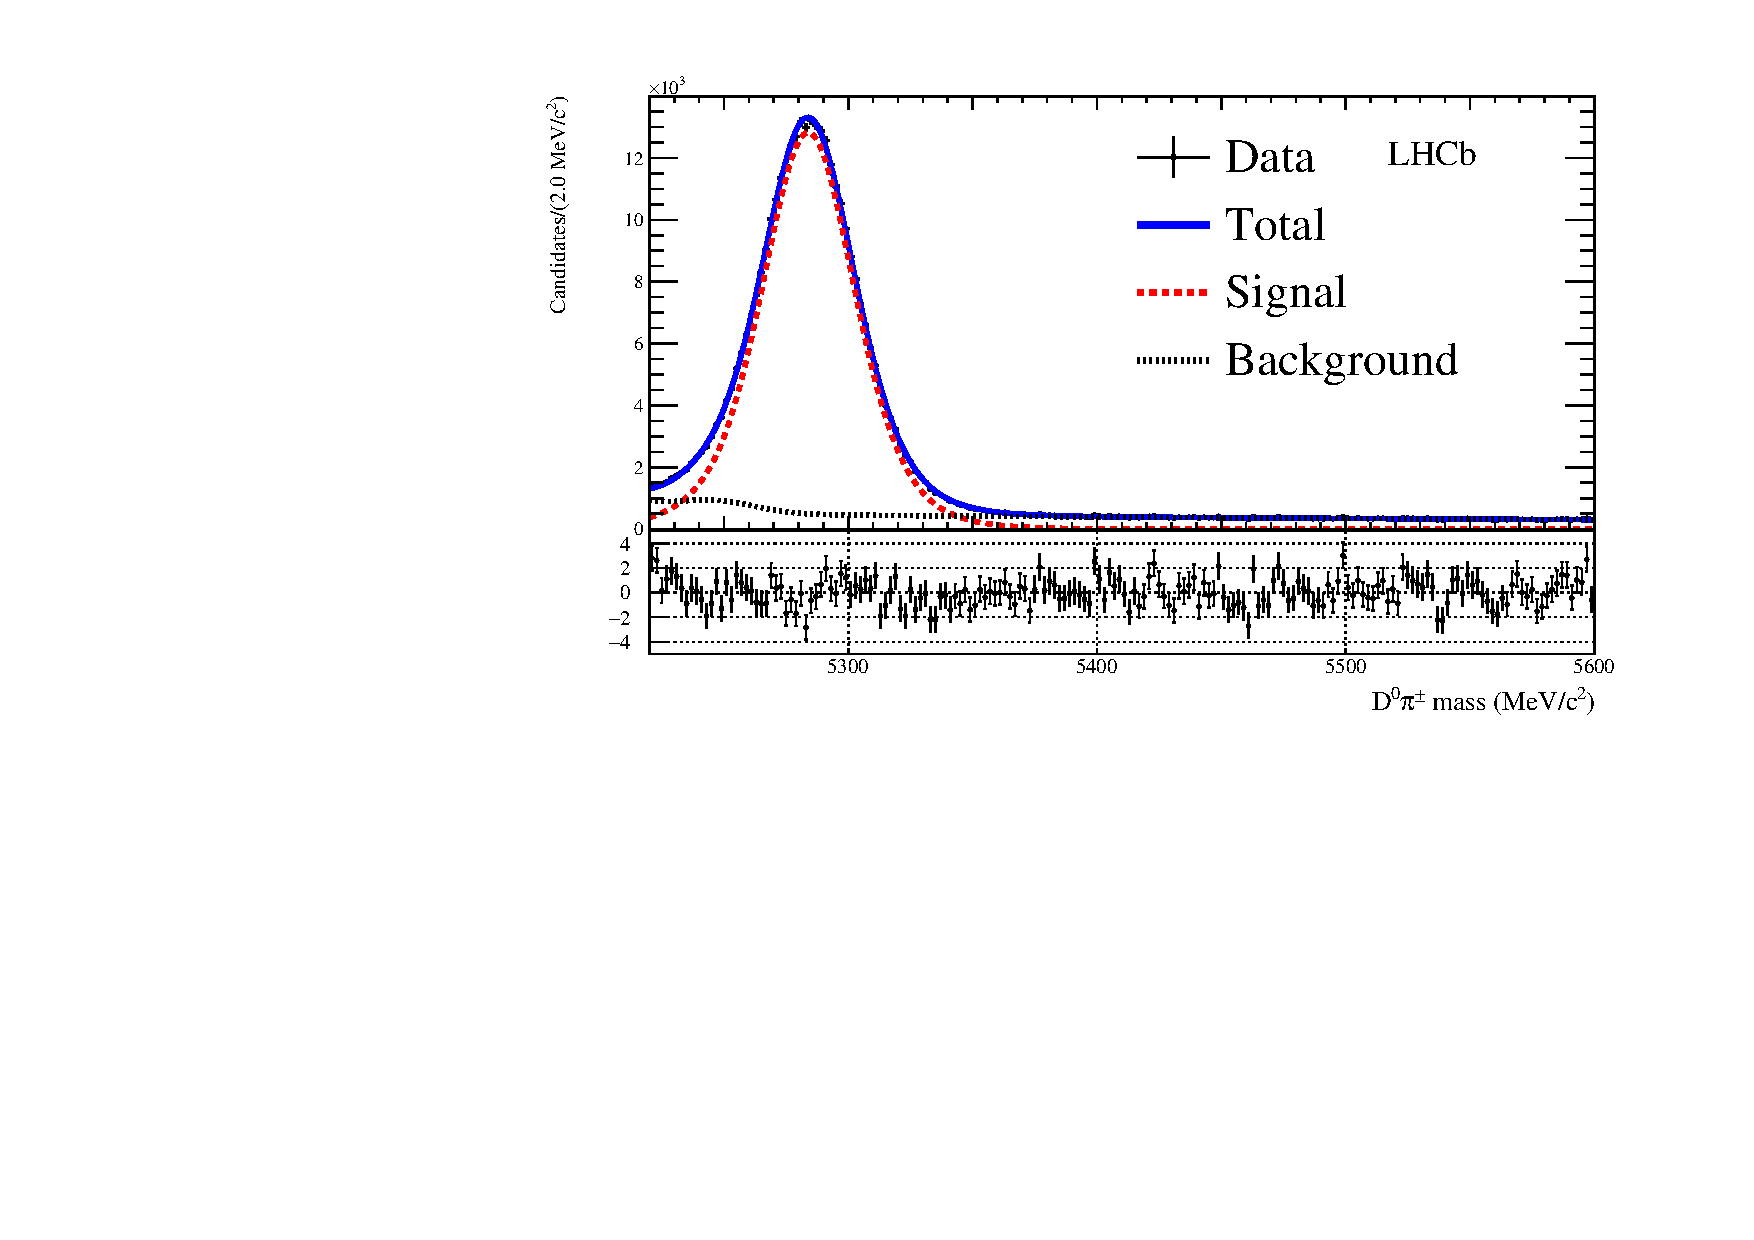
\includegraphics[width=0.49\textwidth]{AA-Appdx-OSTaggers/figs/MDFitForSWeights_BeautyMass_Bu2D0Pi.pdf}
	\end{center}
        \vspace{-2mm}
	\caption{Top left: $\Dzb\pip$ mass distribution of the $\pi$ sample. Top right: $\Dzb\pip$ mass distribution of the $K$ sample.
	The result of the simultaneous fit (Fit A) to both samples is superimposed.
	Bottom: $\Dzb\pip$ mass distribution of the $\pi$ sample with the results of Fit B superimposed.}
	\label{fig:OSmassFit}
\end{figure}

\begin{table}[htbp]
  \begin{center}
    \caption{Results of the $\Bp\to\Dzb\pip$ mass fit (Fit A).}
    \begin{tabular}{cc}
\toprule
   Parameter name & Fitted value \\
\midrule
$\mu^{\pi}_{\Bz\to D\pi\pi}$ & $5132.61\pm0.23$ \\
$s\sigma^{\pi}_{\Bz\to D\pi\pi}$ & $0.780\pm0.015$ \\
$\sigma^{K}_{B^{+}\to DK}$ & $19.47\pm0.30$ \\
$\sigma^{\pi}_{B^{+}\to DK}$ & $16.62\pm0.69$ \\
$\mu^{K}_{B^{+}\to DK^{*}}$ & $4960\pm150$ \\
$\sigma^{K}_{B^{+}\to DK^{*}}$ & $88\pm37$ \\
$c^{K}_{\rm comb}$ & $-0.001305\pm0.000035$ \\
$c1^{\pi}_{\rm comb}$ & $-0.001279\pm0.000022$ \\
$\mu^{K}_{B^{+}\to D\pi}$ & $5283.18\pm0.22$ \\
$\mu^{\pi}_{B^{+}\to D\pi}$ & $5283.880\pm0.046$ \\
$sa^{\pi}_{B^{+}\to D\pi}$ & $0.804\pm0.016$ \\
$\mu^{K}_{B^{+}\to D\pi}$ & $5325.4\pm1.2$ \\
$sn^{\pi}_{B^{+}\to D\pi}$ & $2.70\pm0.94$ \\
$\sigma^{\pi}_{B^{+}\to D\pi}$ & $22.850\pm0.054$ \\
$N^{\pi}_{\Bz\to D\pi\pi}$ & $27245\pm430$ \\
$N^{K}_{B^{+}\to DK}$ & $18030\pm296$ \\
$N^{K}_{LM}$ & $5154\pm944$ \\
$N^{K}_{B^{+}\to D^{*}\pi}$ & $5704\pm1350$ \\
$N^{\pi}_{B^{+}\to D^{*}\pi}$ & $41871\pm578$ \\
$N^{K}_{\rm comb}$ & $58761\pm555$ \\
$N^{\pi}_{\rm comb}$ & $146824\pm793$ \\
$N^{\pi}_{B^{+}\to D\pi}$ & $322597\pm812$ \\
\bottomrule
    \end{tabular}
    \label{tab:OSmassFitA}
  \end{center}
\end{table}

\begin{table}[htbp]
  \begin{center}
    \caption{Results of the $\Bp\to\Dzb\pip$ mass fit (Fit B).}
    \begin{tabular}{cc}
      \toprule
    Parameter & Fitted value \\
    \midrule
    $N^{\pi}_{\rm bkg}$ & $85\,687\pm377$ \\
    $N^{\pi}_{B^{+}\to D\pi}$ & $319\,974\pm612$ \\
    \bottomrule
    \end{tabular}
    \label{tab:OSmassFitB}
  \end{center}
\end{table}

\subsection[Reweighting of $\Bp\to\Dzb\pip$ to $\Bz\to\Dmp\pipm$]{Reweighting of \boldmath{$\Bp\to\Dzb\pip$} to \boldmath{$\Bz\to\Dmp\pipm$}}
\label{app:ReweightingOSTagging}

In order to improve the OS calibration portability, a multi-dimensional reweighting of the \emph{sWeighted} $\Bp\to\Dzb\pip$ distributions
is made to match the $\Bz\to\Dmp\pipm$ kinematics.

The reweighting is made in two steps. In the first step, the variables considered in the reweighting are 
the transverse momentum, the pseudo-rapidity $\eta$ and the decay time $\tau_{B}$ of the $B$ candidate, as well as the
number of tracks and the number of primary vertices of the events. A BDT-based approach is followed in order to cope with 
the high dimensionality of the space as well as with the correlations among variables~\cite{hepml}. A comparison between 
weighted and unweighted distributions is provided in Figs.~\ref{fig:reweightingOSgb1} and \ref{fig:reweightingOSgb2}. 

\begin{figure}[t]
  \begin{center}
   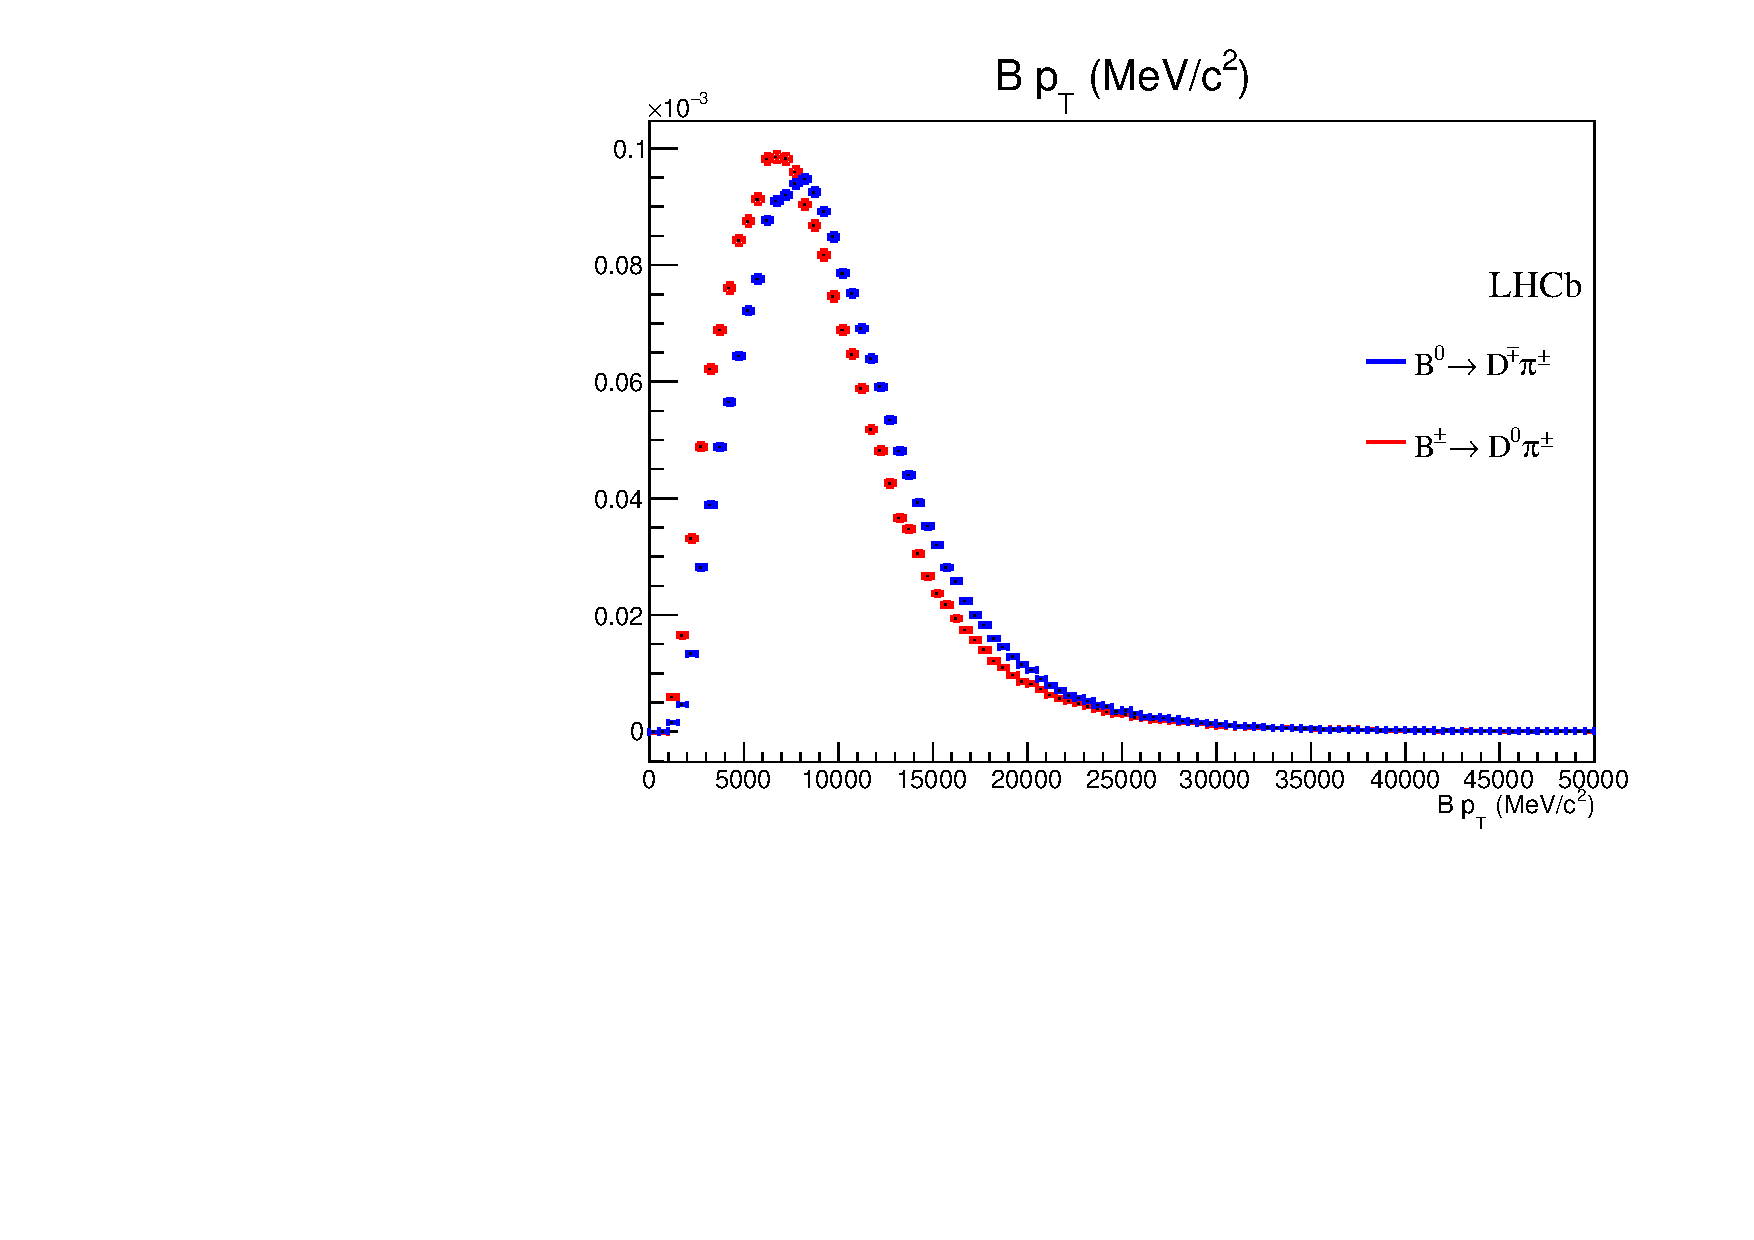
\includegraphics[width=0.49\textwidth]{AA-Appdx-OSTaggers/figs/BPT_BuVSBd_Unweighted.pdf}
   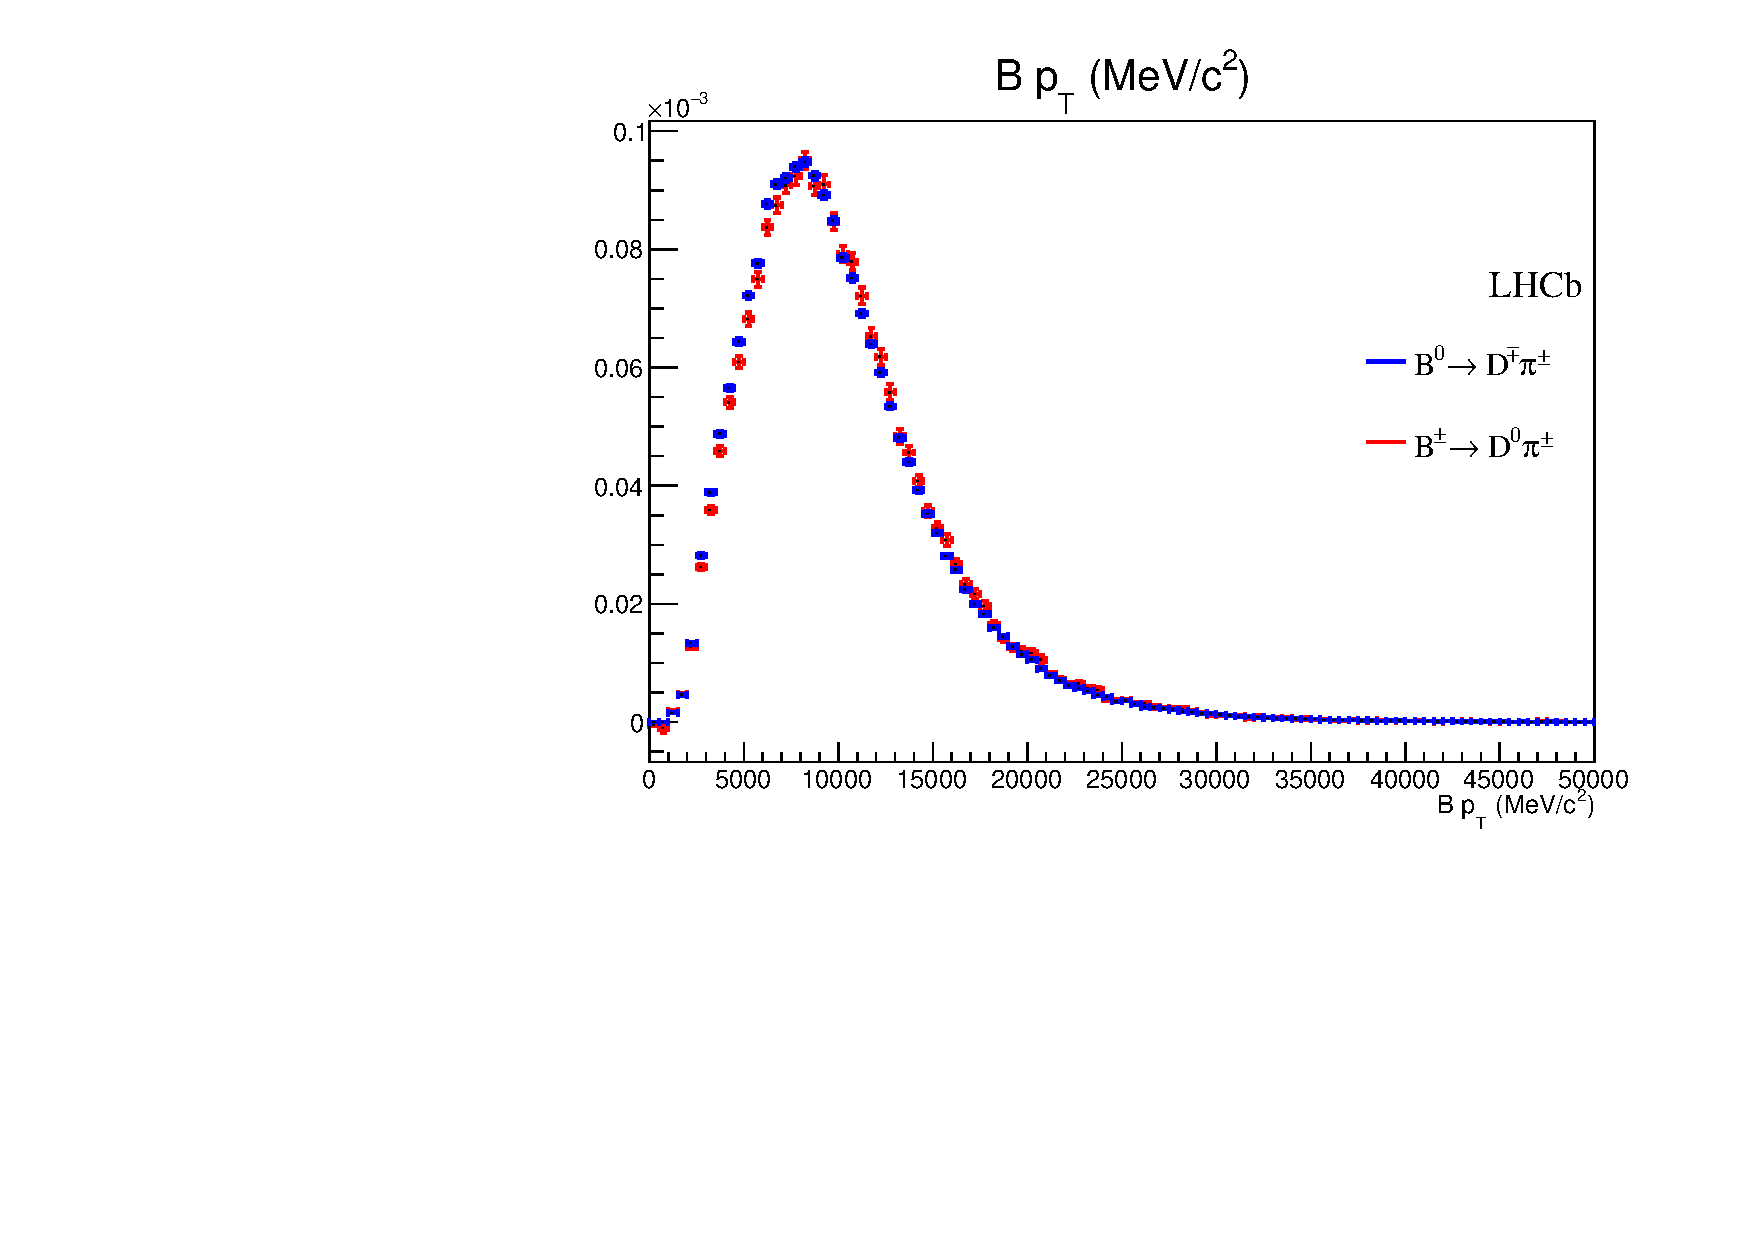
\includegraphics[width=0.49\textwidth]{AA-Appdx-OSTaggers/figs/BPT_BuVSBd_Weighted.pdf} \\
   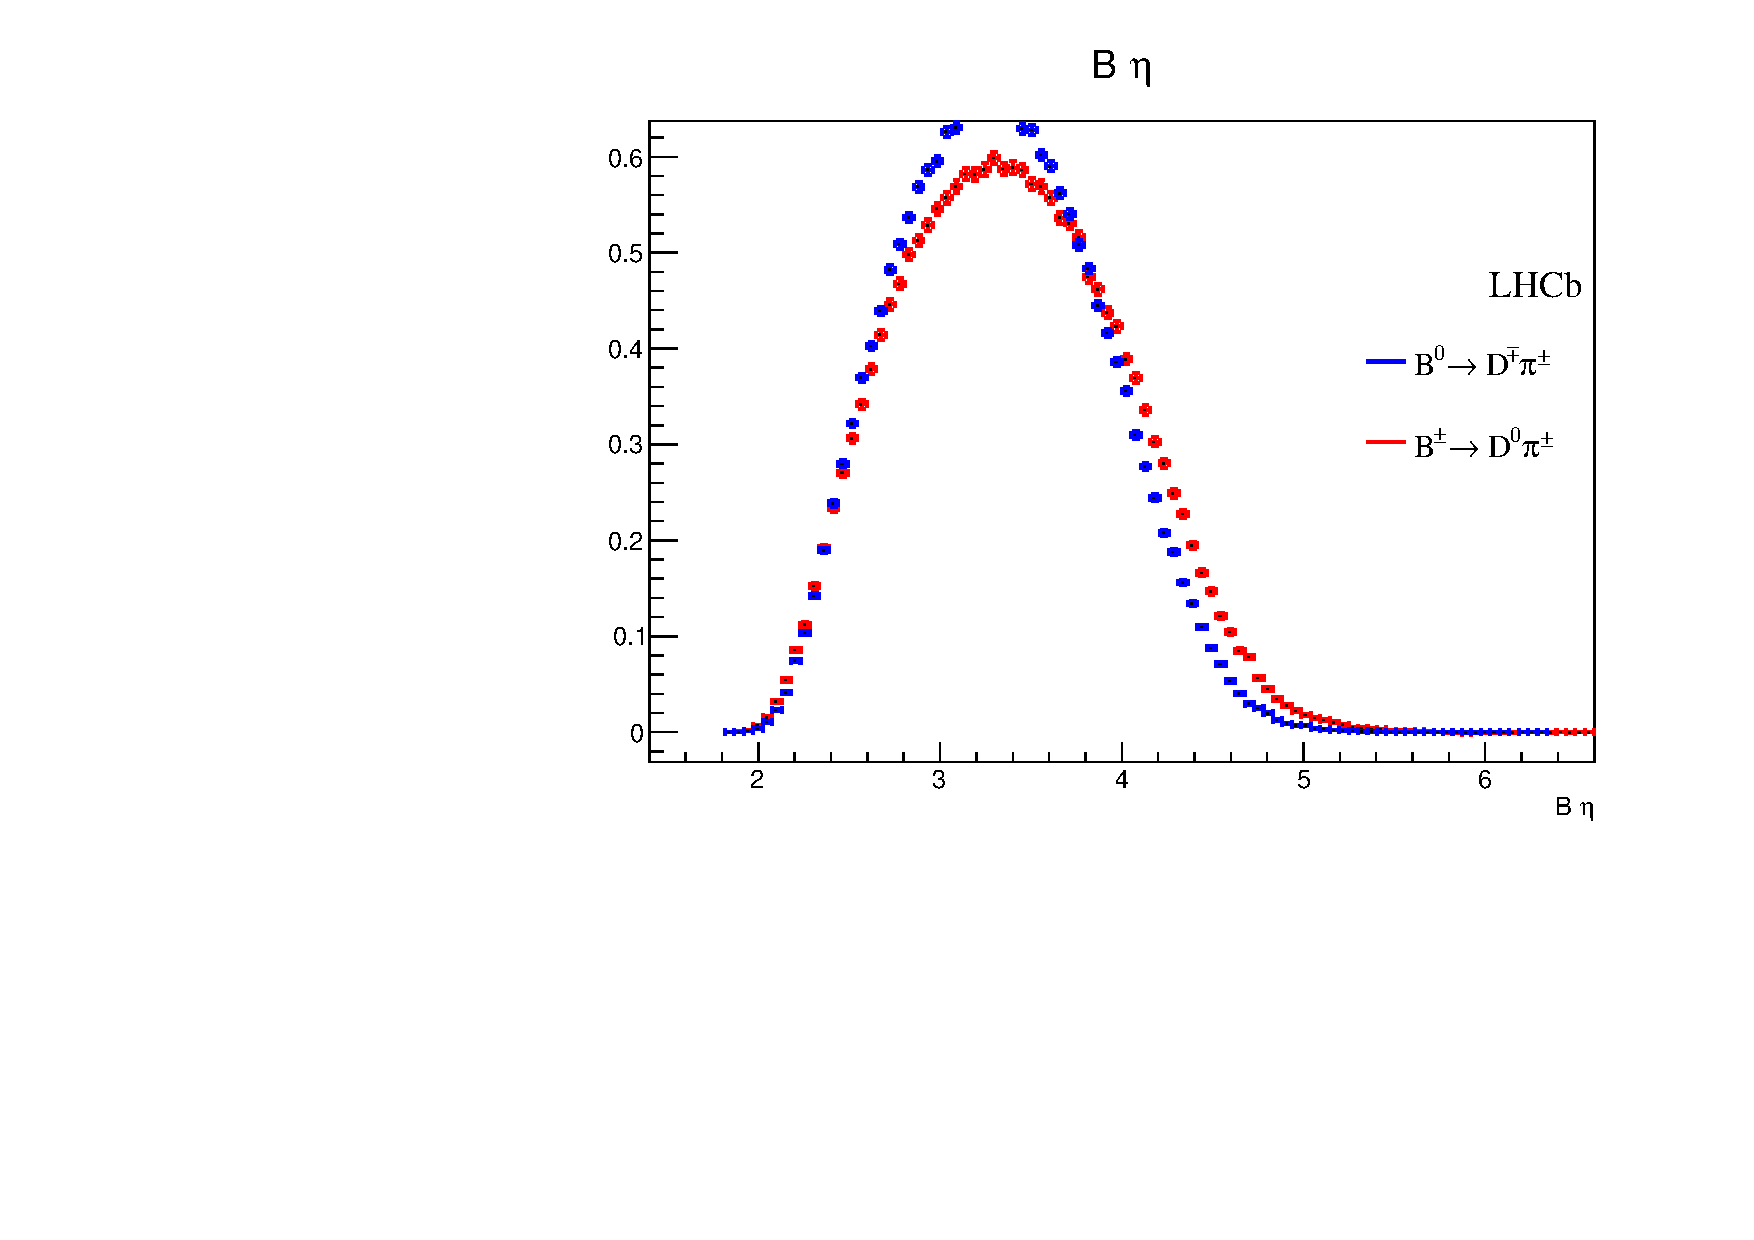
\includegraphics[width=0.49\textwidth]{AA-Appdx-OSTaggers/figs/BETA_BuVSBd_Unweighted.pdf}
   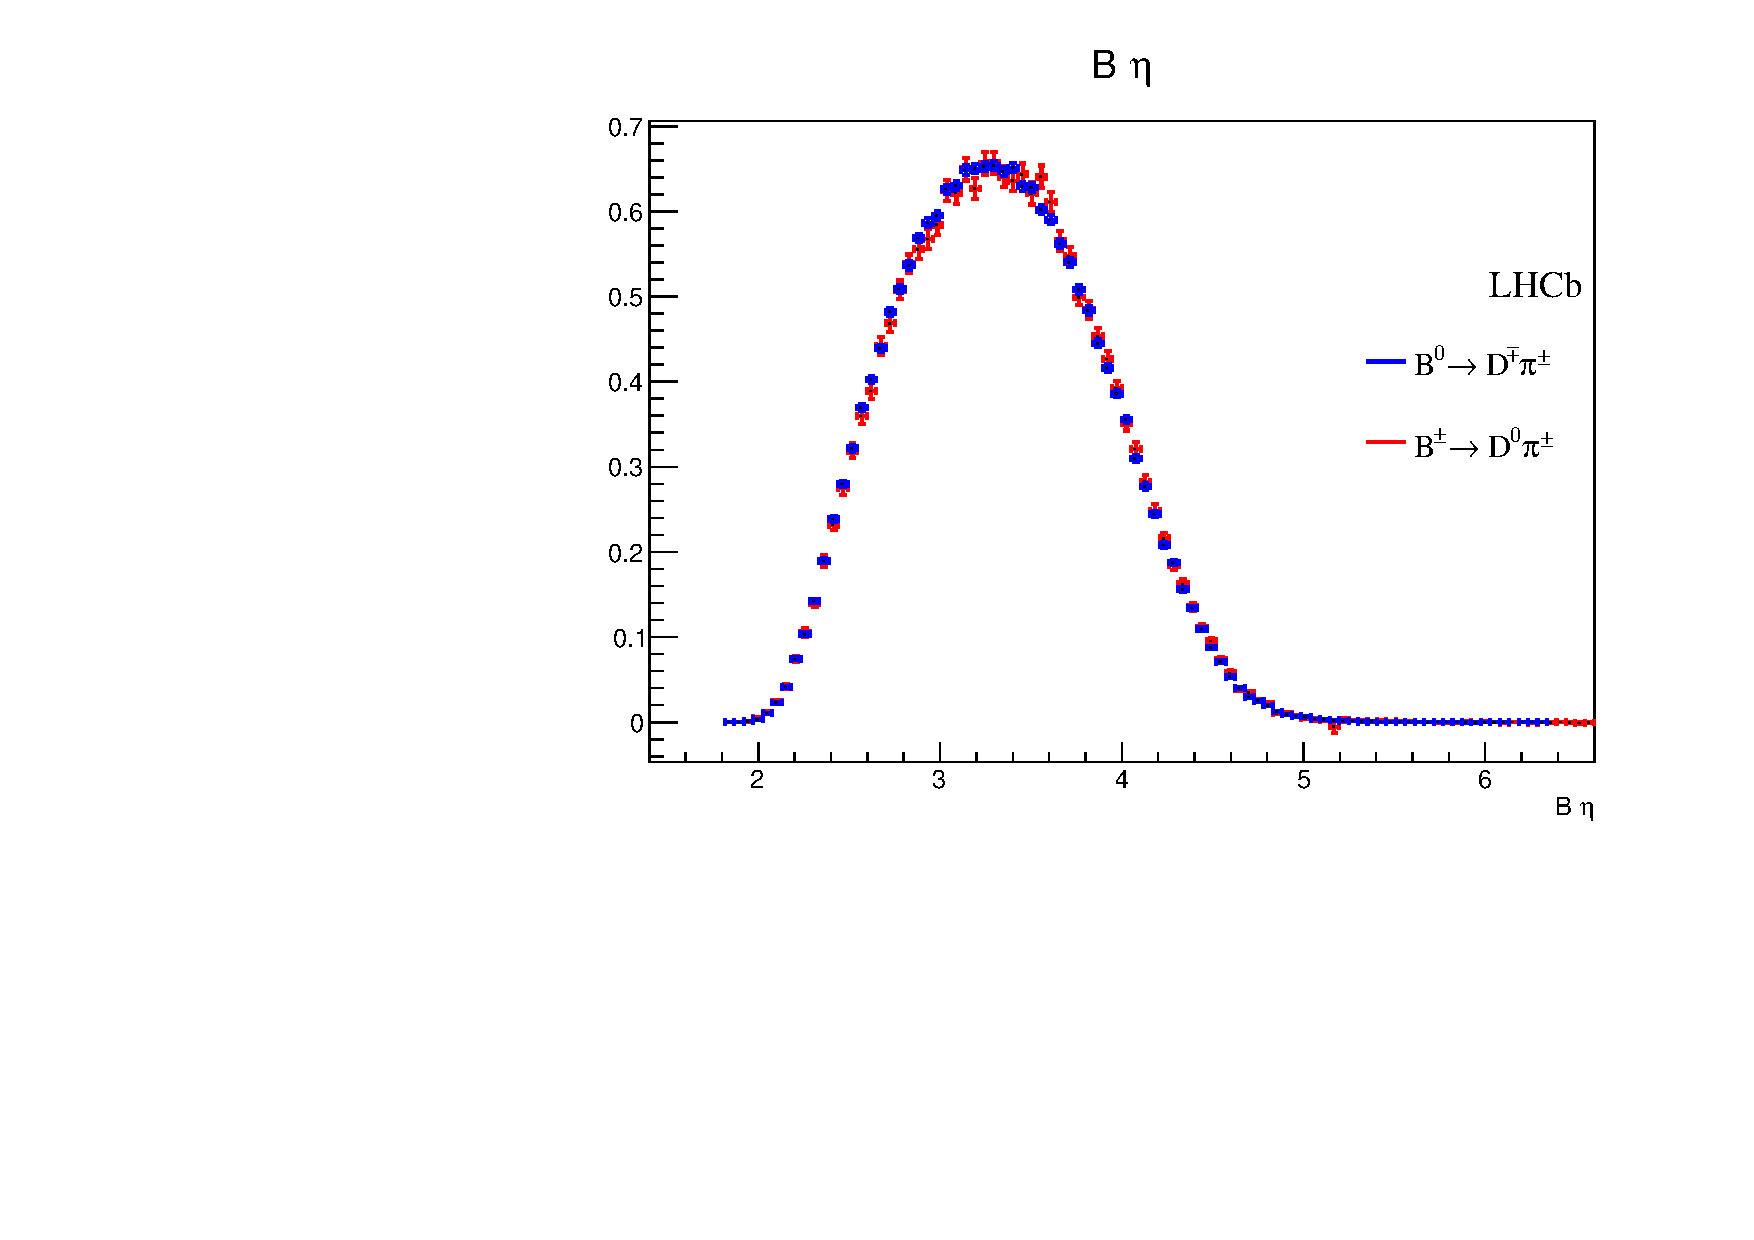
\includegraphics[width=0.49\textwidth]{AA-Appdx-OSTaggers/figs/BETA_BuVSBd_Weighted.pdf} \\
   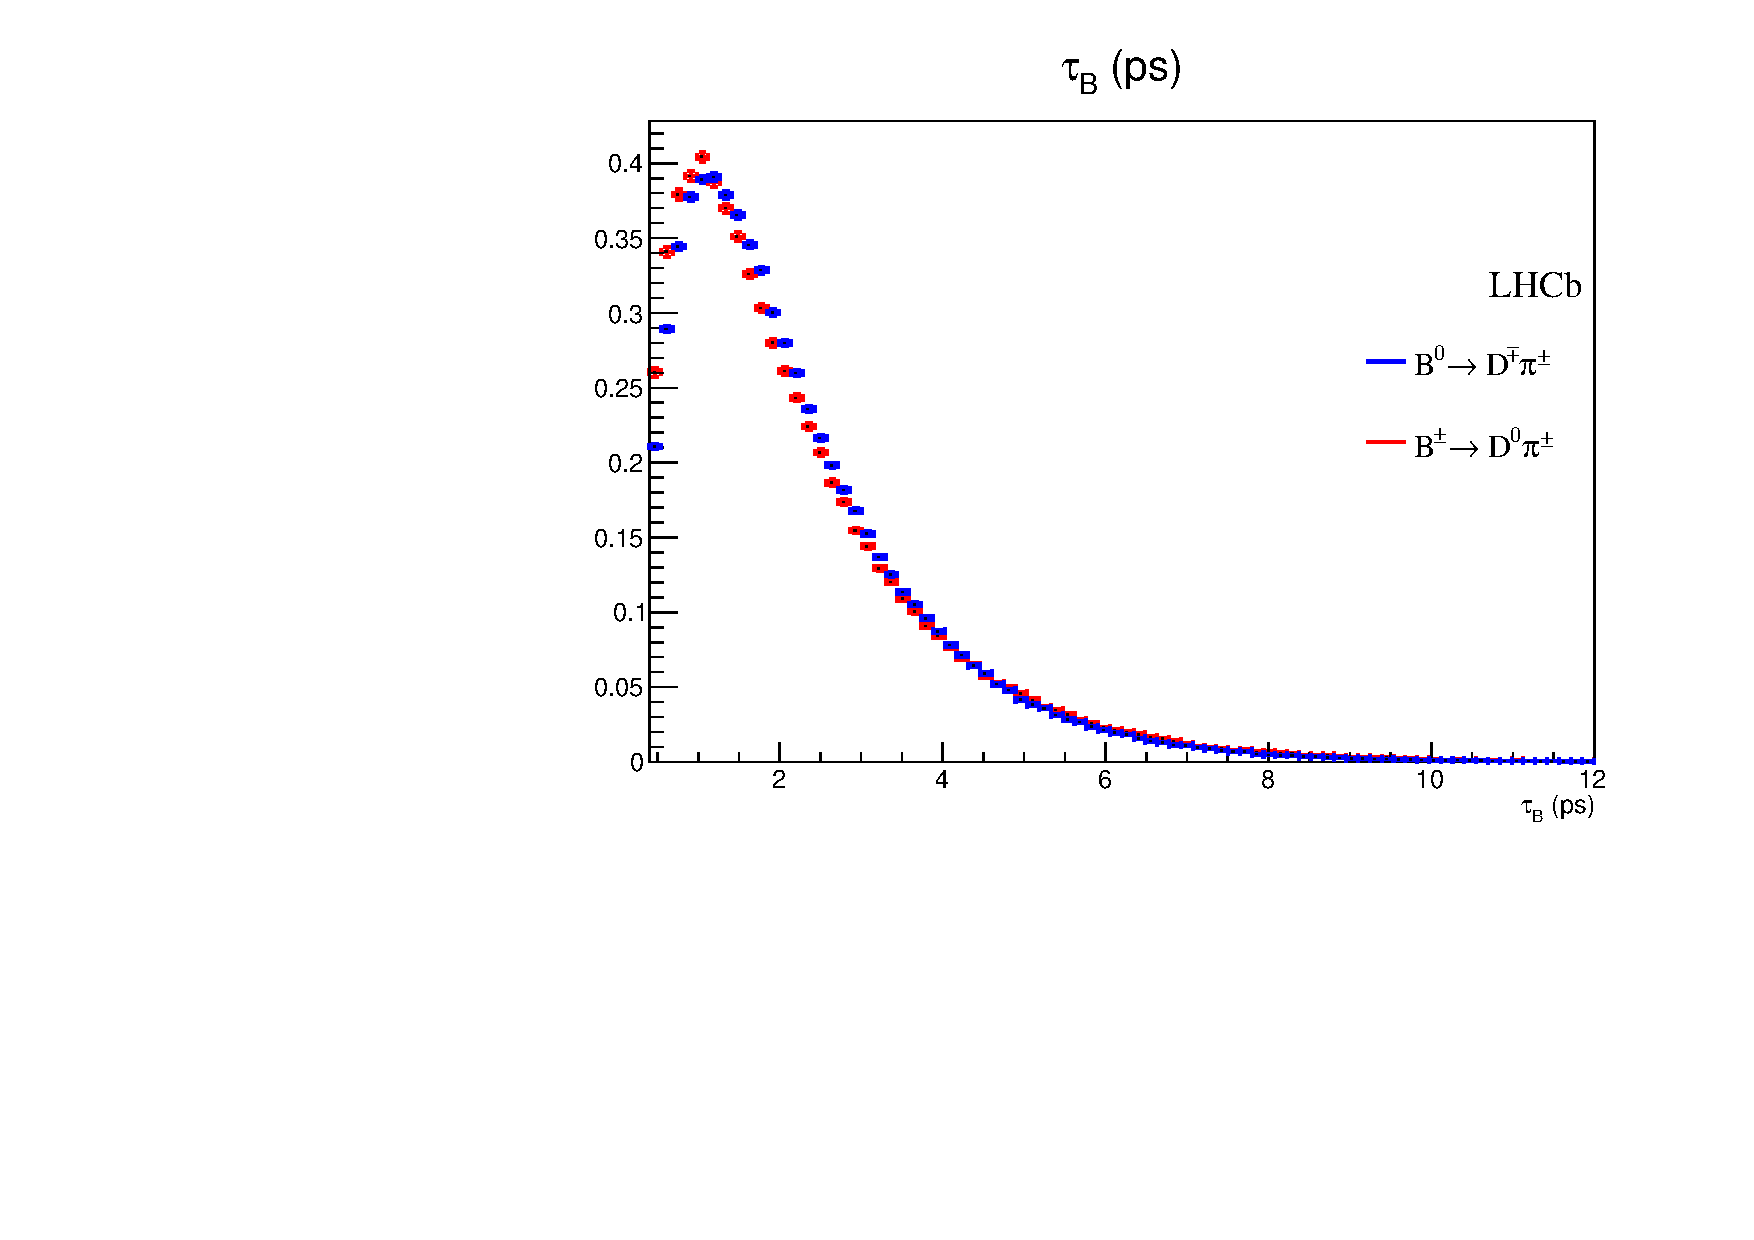
\includegraphics[width=0.49\textwidth]{AA-Appdx-OSTaggers/figs/BTAU_BuVSBd_Unweighted.pdf}
   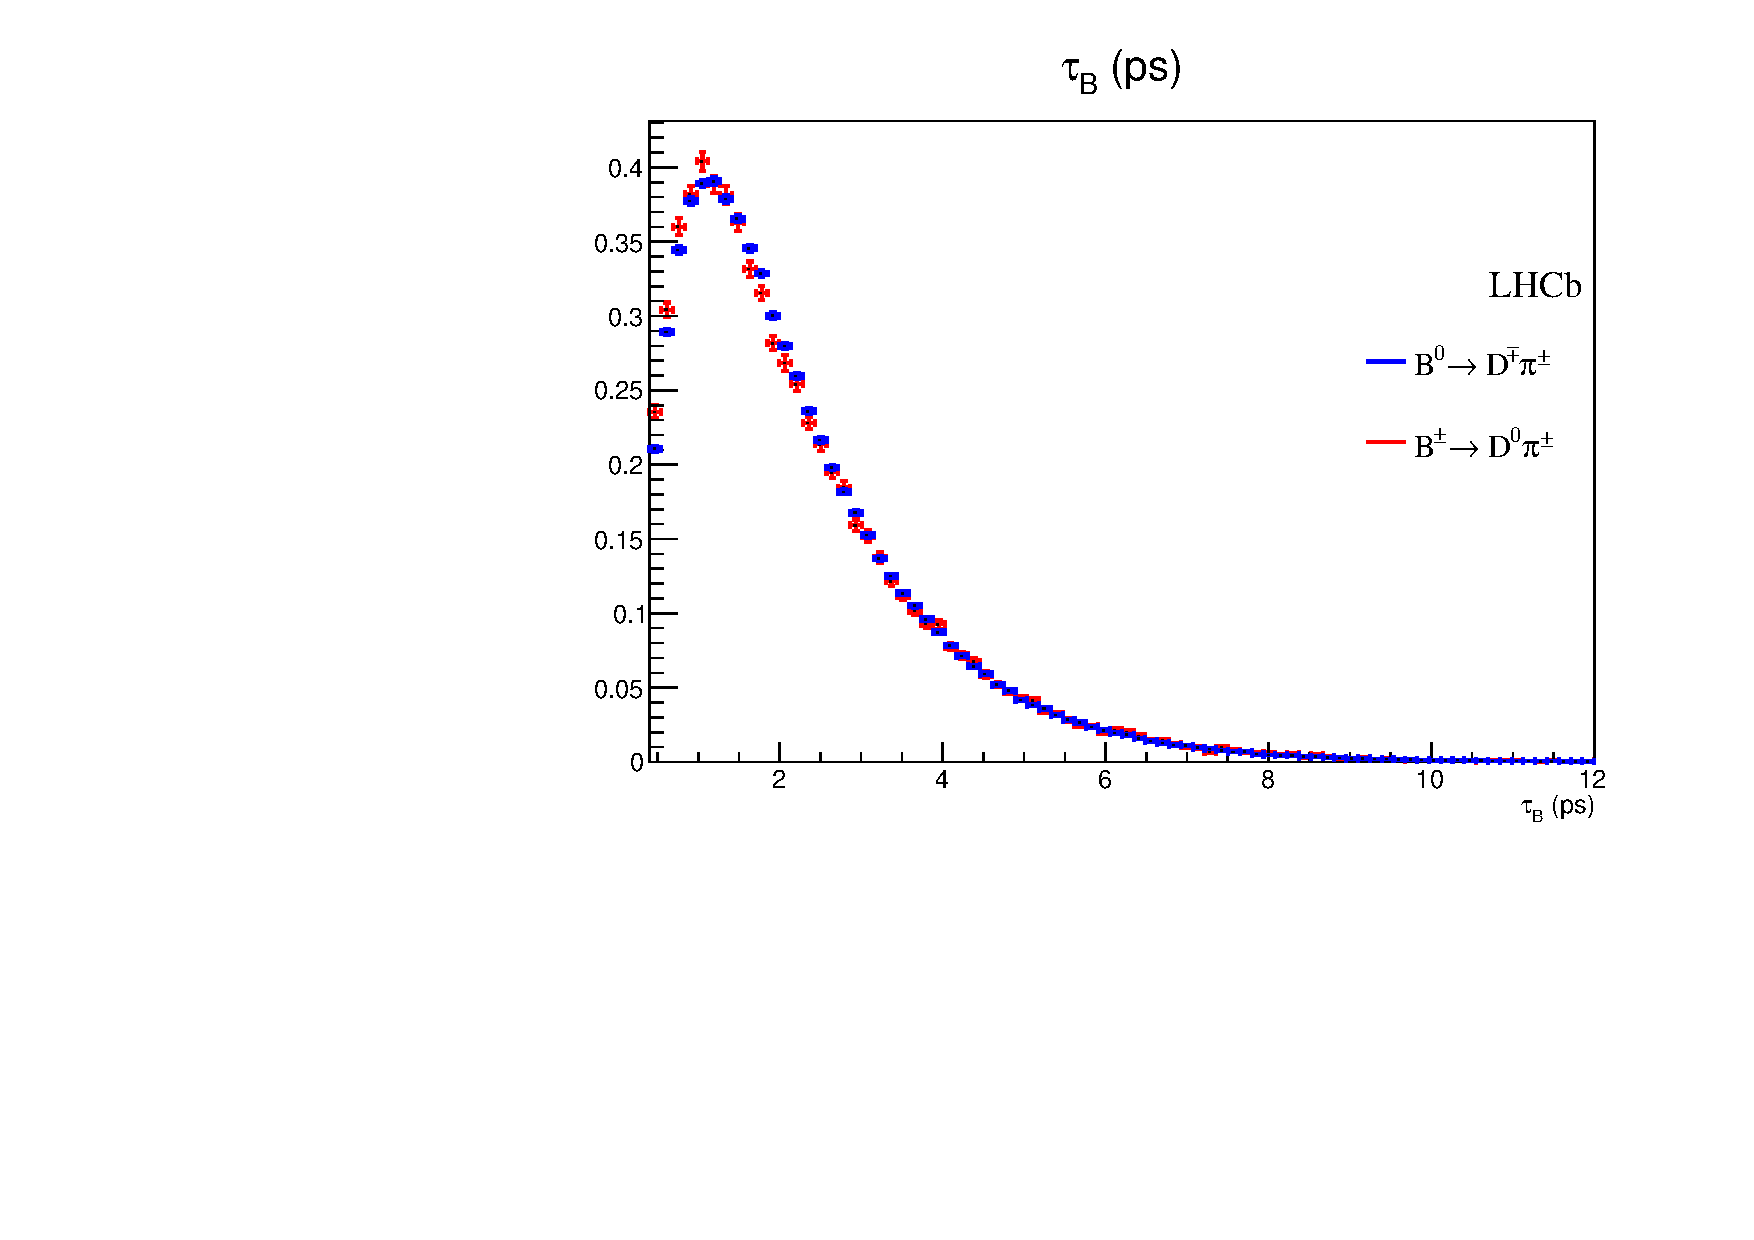
\includegraphics[width=0.49\textwidth]{AA-Appdx-OSTaggers/figs/BTAU_BuVSBd_Weighted.pdf} \\
  \end{center}
  \vspace{-2mm}
  \caption{Normalised \emph{sWeighted} distributions of the transverse momentum, the pseudo-rapidity $\eta$ and the decay time $\tau_{B}$ of the $\Bz$ and $\Bp$ mesons. Left: unweighted distributions. Right: distributions after reweighting the $\Bp\to\Dzb\pip$ events.}
  \label{fig:reweightingOSgb1}
\end{figure}
\begin{figure}[t]
  \begin{center}
   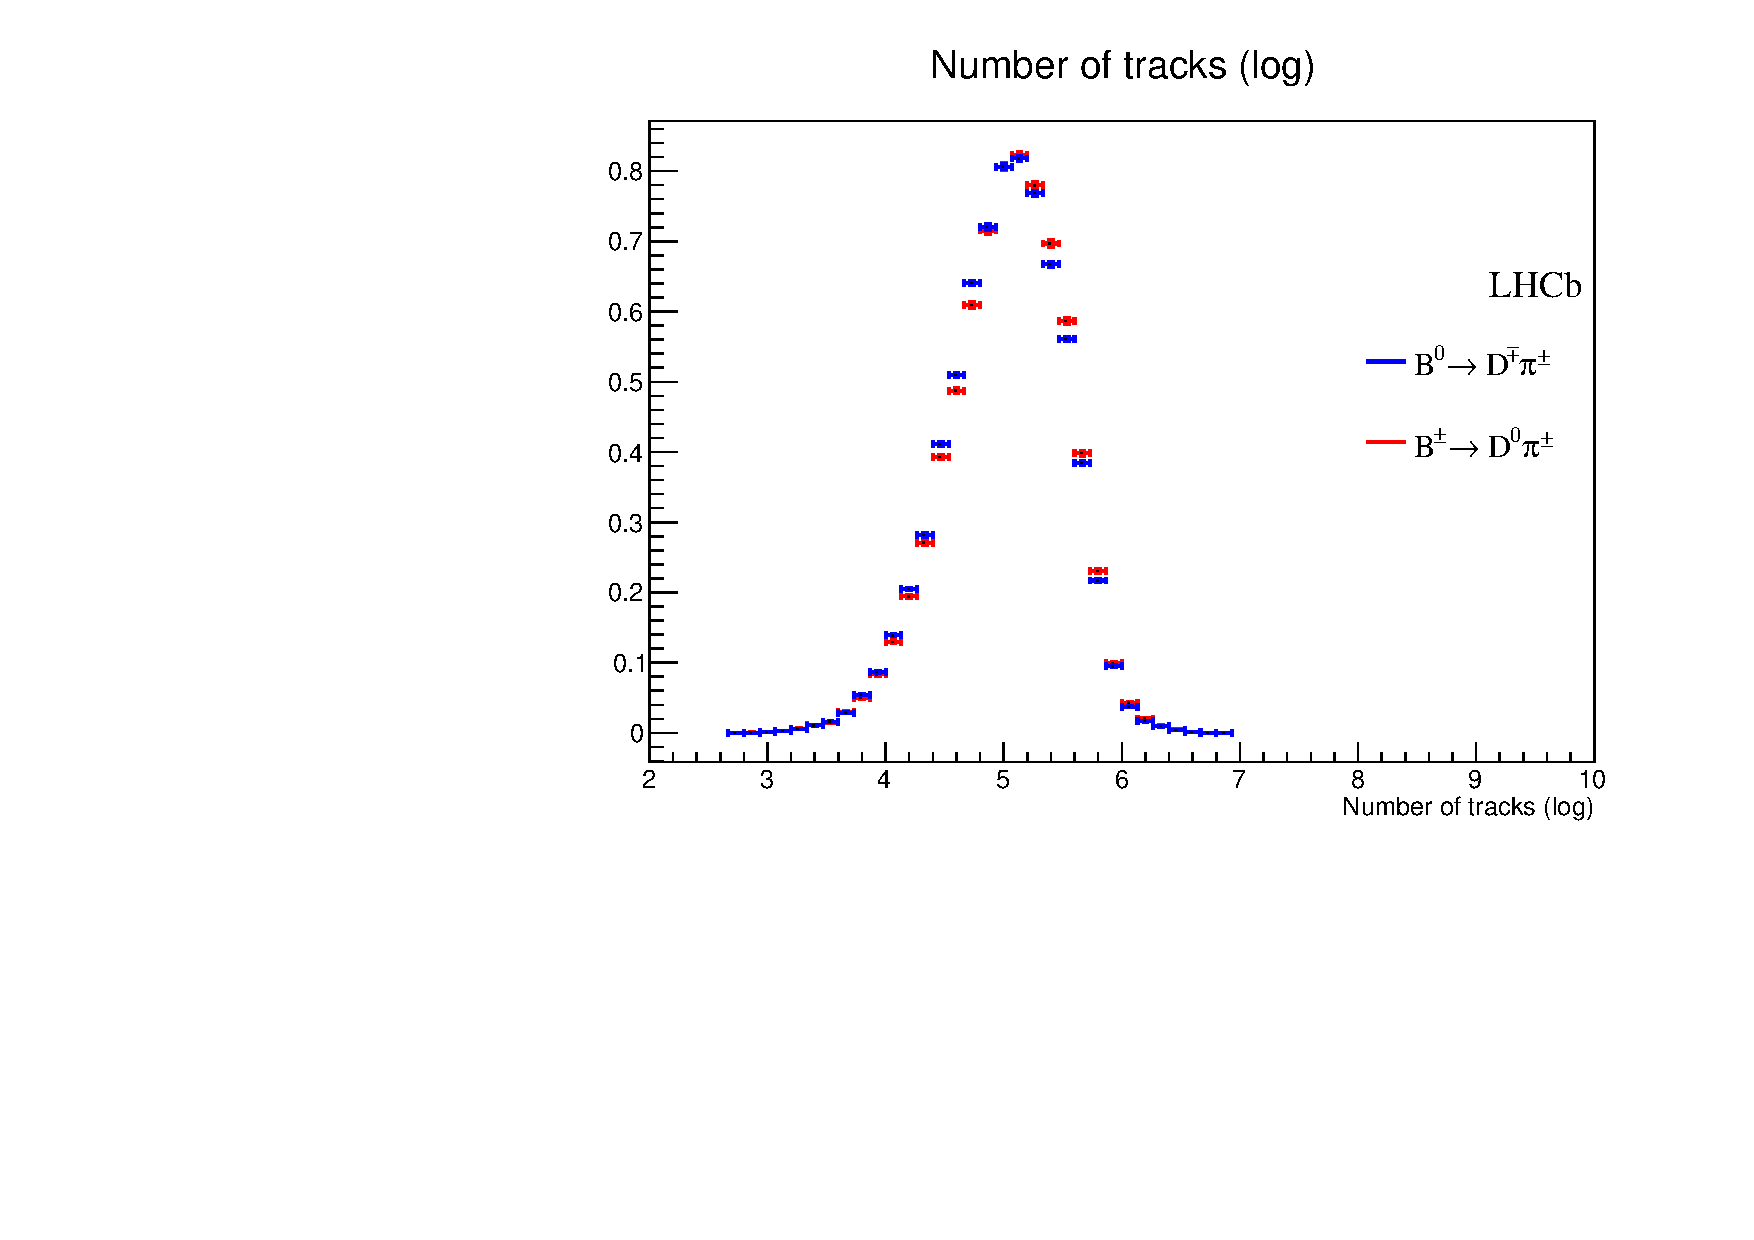
\includegraphics[width=0.49\textwidth]{AA-Appdx-OSTaggers/figs/nTracks_BuVSBd_Unweighted.pdf}
   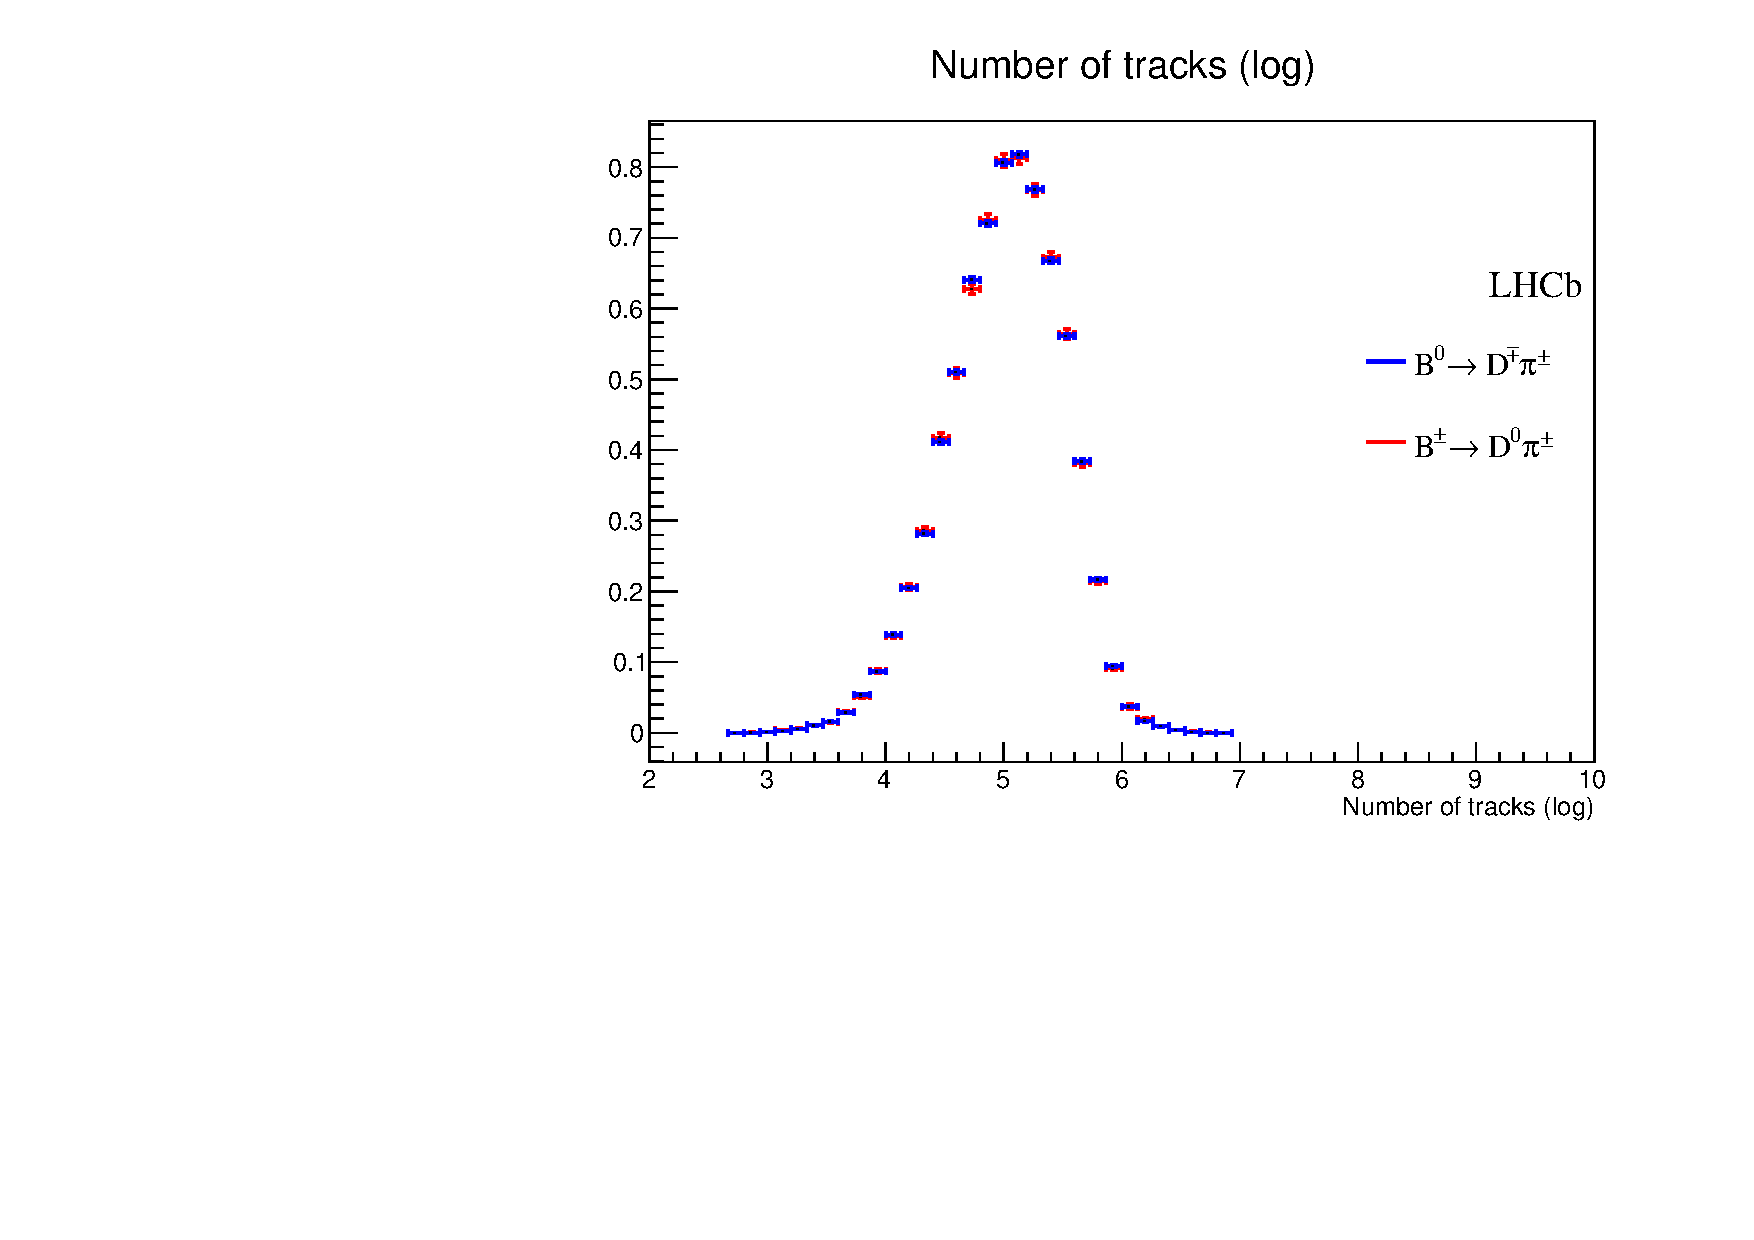
\includegraphics[width=0.49\textwidth]{AA-Appdx-OSTaggers/figs/nTracks_BuVSBd_Weighted.pdf} \\
   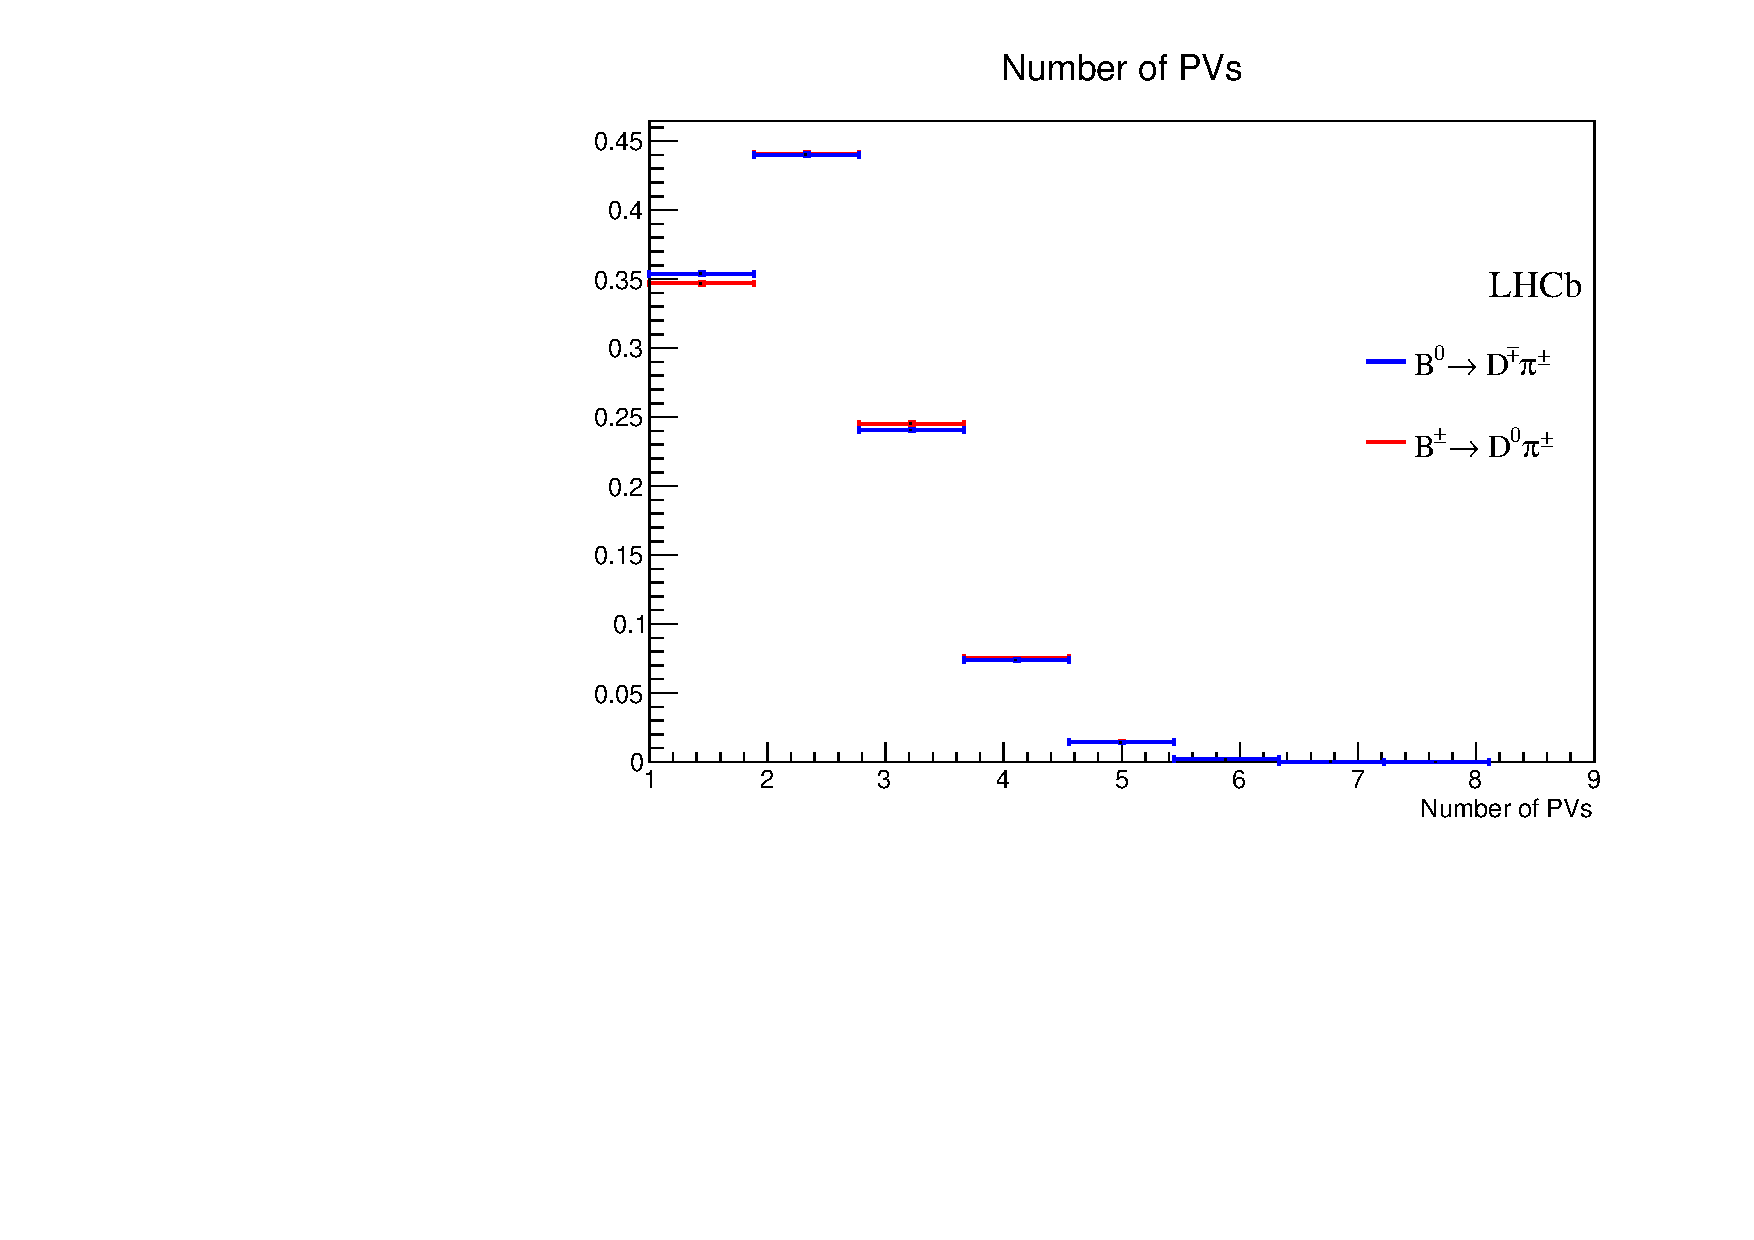
\includegraphics[width=0.49\textwidth]{AA-Appdx-OSTaggers/figs/nPV_BuVSBd_Unweighted.pdf}
   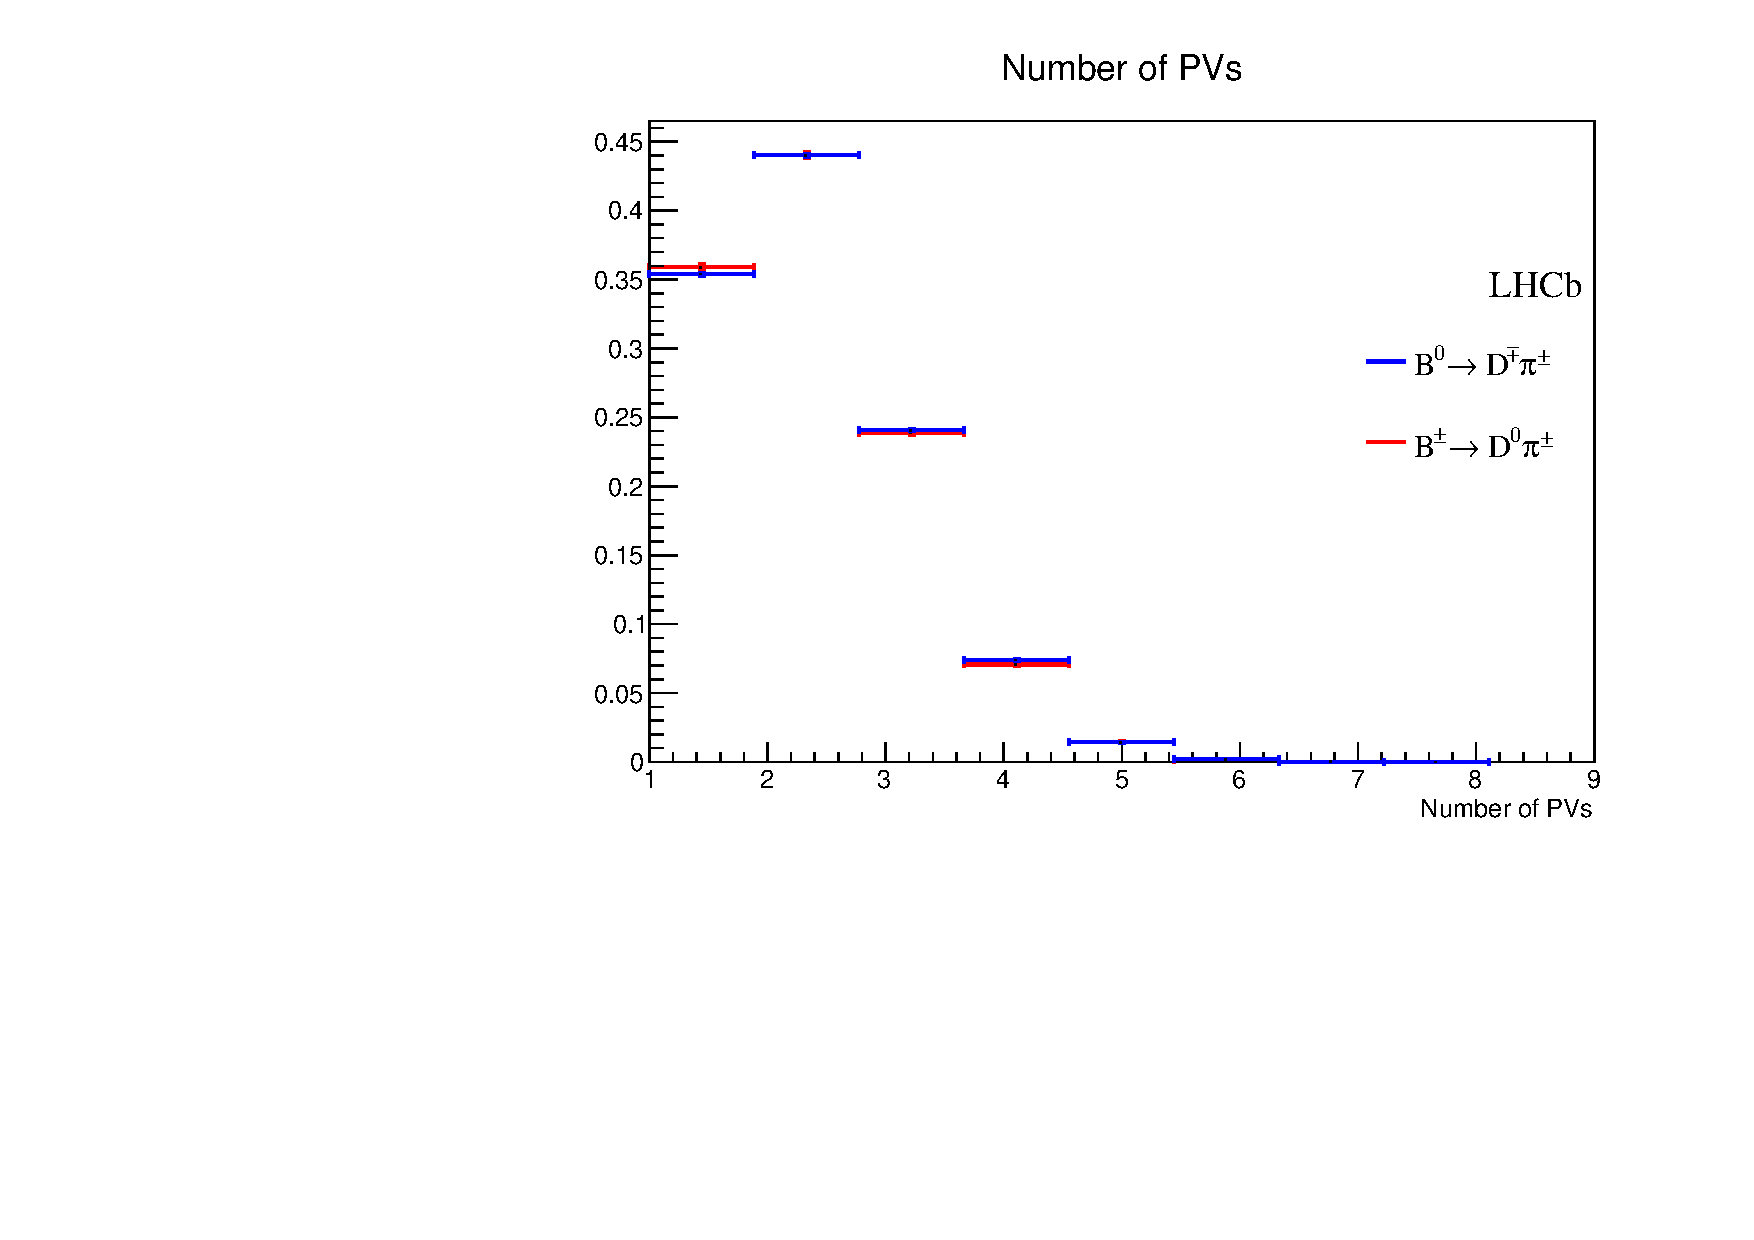
\includegraphics[width=0.49\textwidth]{AA-Appdx-OSTaggers/figs/nPV_BuVSBd_Weighted.pdf}\\
  \end{center}
  \vspace{-2mm}
  \caption{Normalised \emph{sWeighted} distributions of the number of tracks and PVs in a $\Bz$ or $\Bp$ event. Left: unweighted distribution. Right: distributions after reweighting the $\Bp\to\Dzb\pip$ events.}
  \label{fig:reweightingOSgb2}
\end{figure}

In the second step, a new weight is computed by comparing the two-dimensional distributions of the $D$ meson decay time and HLT2 trigger composition between $\Bp\to\Dzb\pip$ and $\Bz\to\Dmp\pipm$ after \emph{sWeights} and the weights from the first step are applied. The HLT2 composition observable is a categorical variable which describes which HLT2 trigger line has been fired by the $B$ candidate:
\begin{itemize}[noitemsep,topsep=0pt]
  \item \verb!Hlt2Topo2BodyBBDTDecision! only (value $0$);
  \item \verb!Hlt2Topo3BodyBBDTDecision! or \verb!Hlt2Topo4BodyBBDTDecision! only (value $1$);
  \item overlap of the first two categories (value $2$). 
\end{itemize} 
This reweighting is done separately from the first one in order to avoid a too fine partition of the samples, which would result in very low statistics in less populated bins. The reason why HLT2 trigger and $D$ decay time are reweighted simultaneously is that these two observables are correlated.
The result of this second reweighting is shown in Fig.~\ref{fig:reweightingOSsecond}.

\begin{figure}[t]
  \begin{center}
   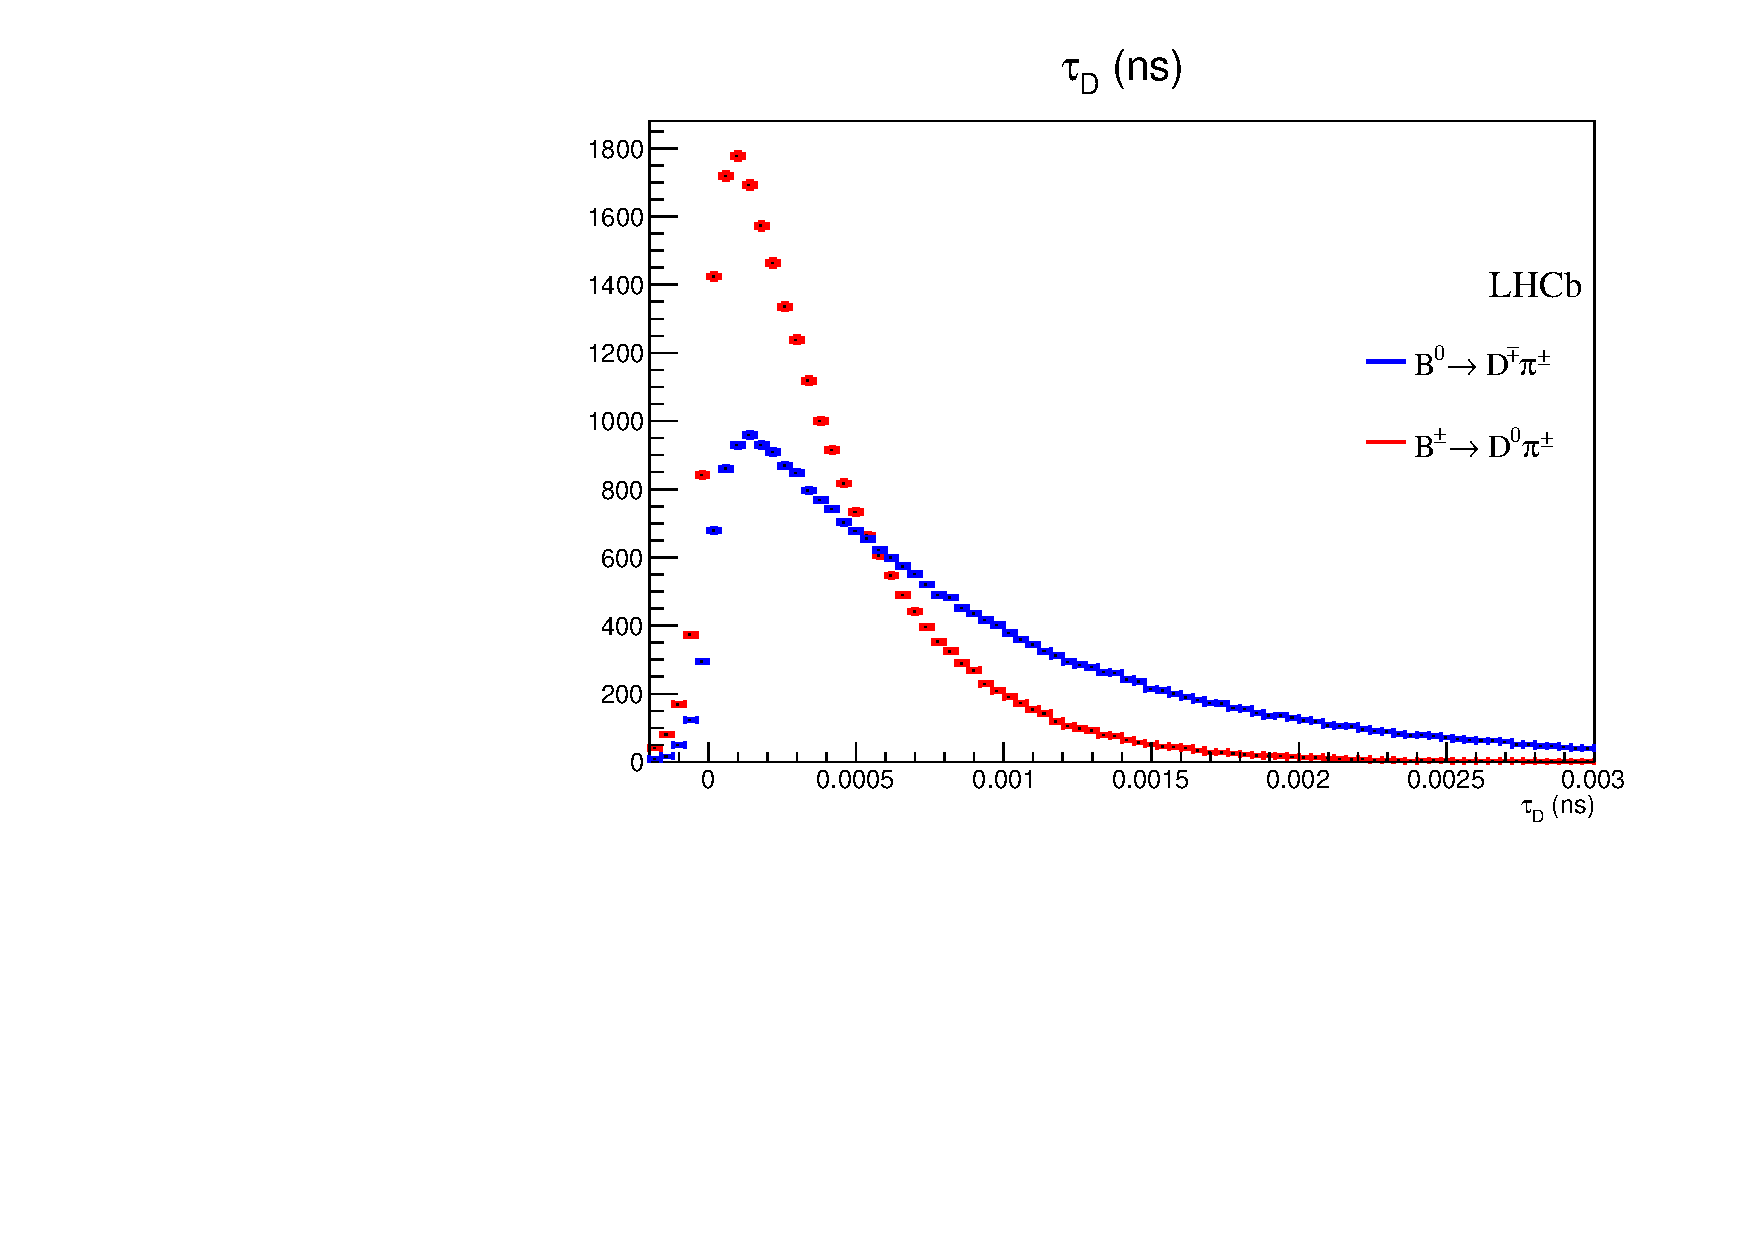
\includegraphics[width=0.49\textwidth]{AA-Appdx-OSTaggers/figs/DTAU_BuVSBd_Unweighted.pdf}
   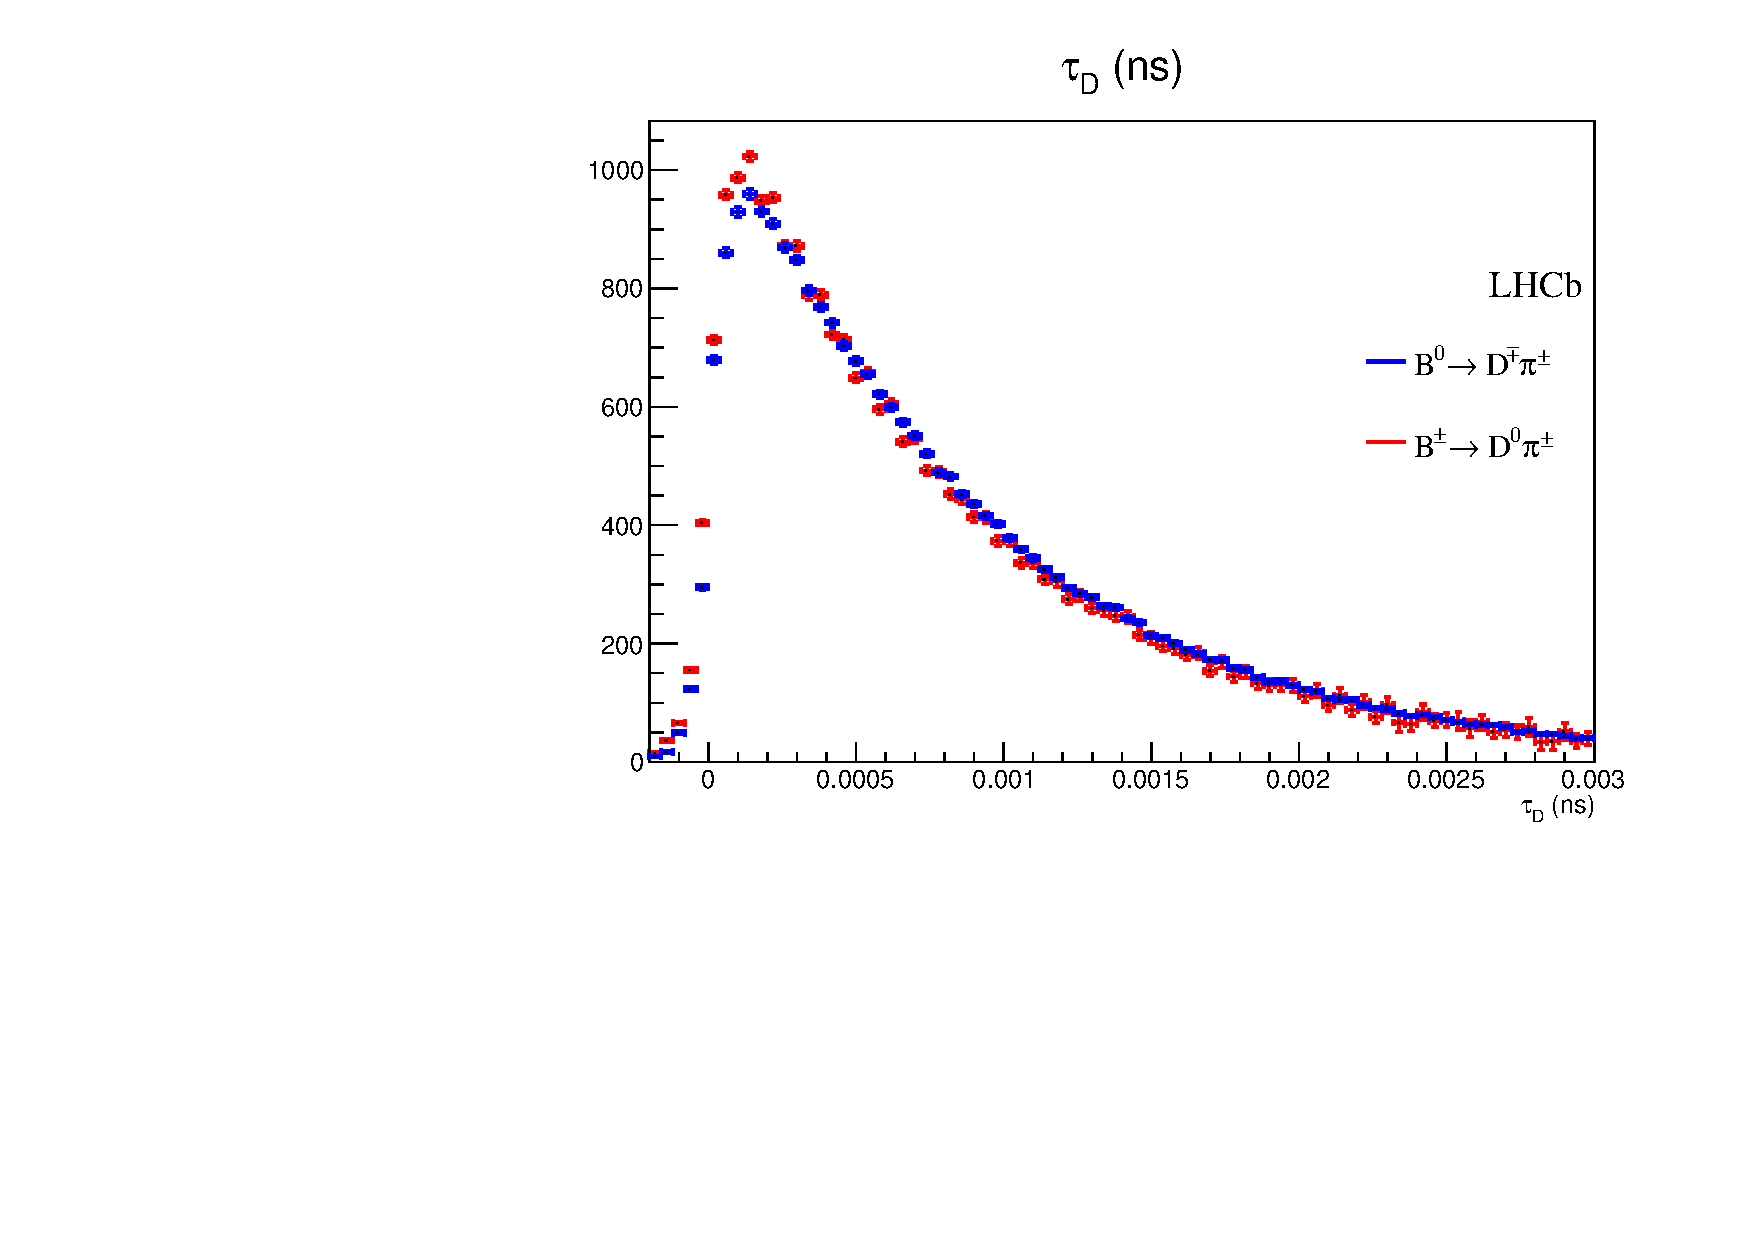
\includegraphics[width=0.49\textwidth]{AA-Appdx-OSTaggers/figs/DTAU_BuVSBd_Weighted.pdf} \\
   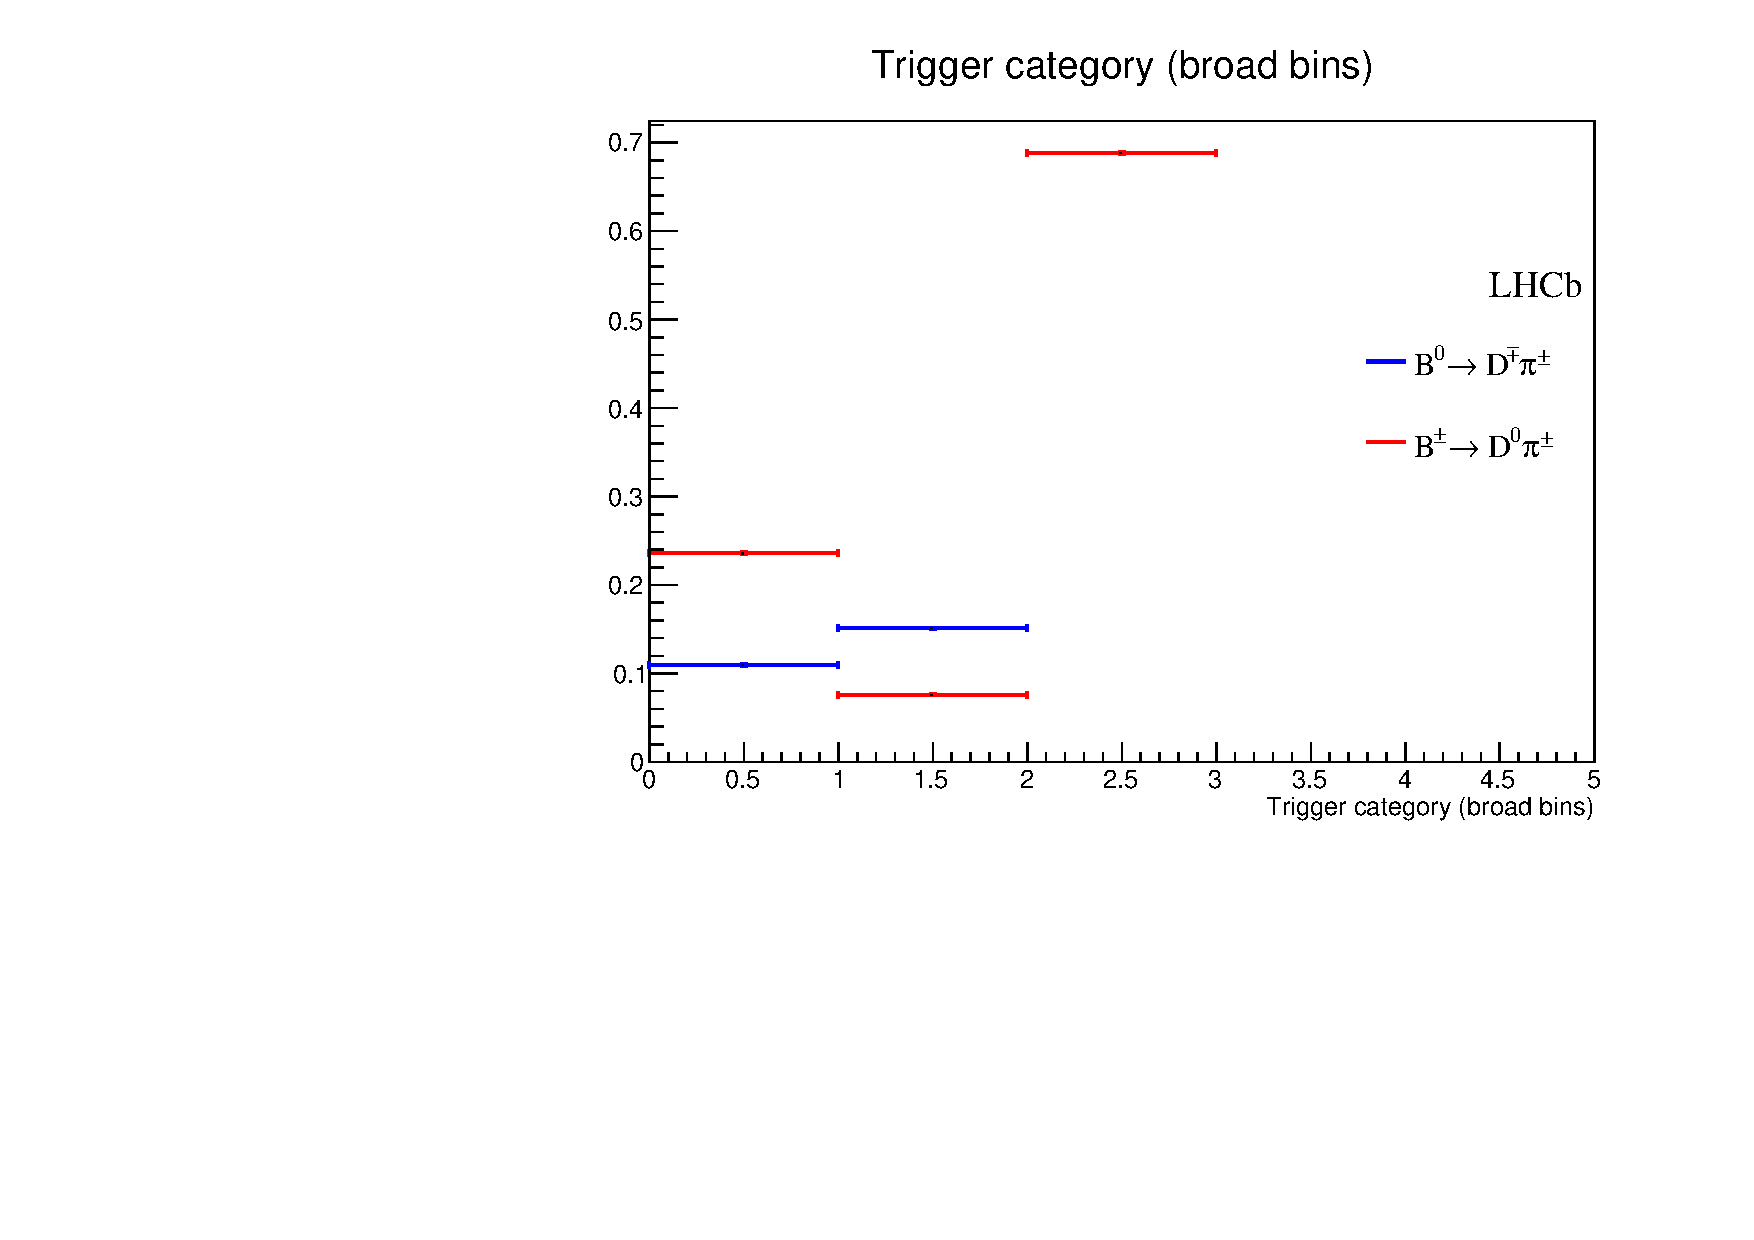
\includegraphics[width=0.49\textwidth]{AA-Appdx-OSTaggers/figs/TRIGCATB_BuVSBd_Unweighted.pdf}
   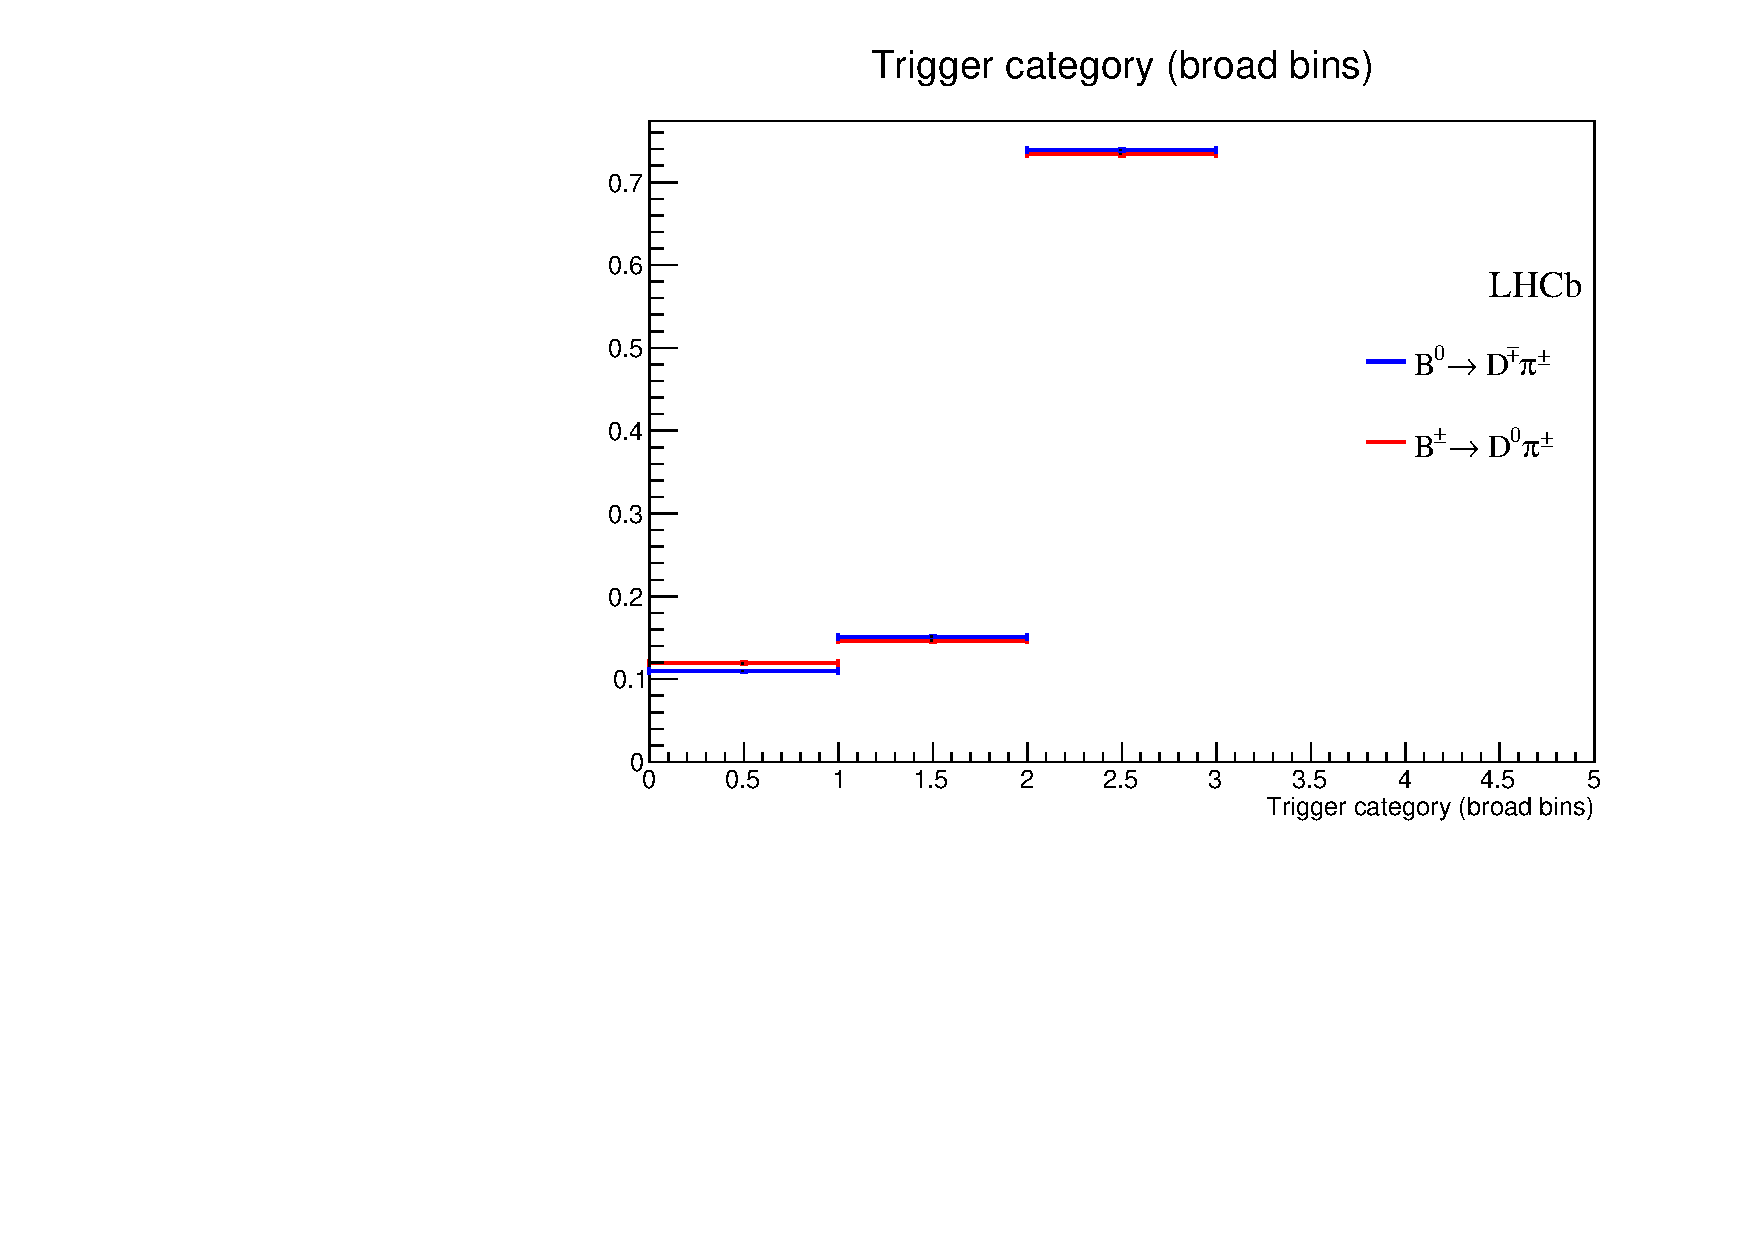
\includegraphics[width=0.49\textwidth]{AA-Appdx-OSTaggers/figs/TRIGCATB_BuVSBd_Weighted.pdf} \\
  \end{center}
  \vspace{-2mm}
  \caption{Normalised \emph{sWeighted} distributions of the $\Dmp$ and $\Dzb$ mesons decay time and HLT2 trigger composition, where the weight obtained from the first reweighting step is also applied. Left: unweighted distributions. Right: distributions after reweighting the $\Bp\to\Dzb\pip$ events.}
  \label{fig:reweightingOSsecond}
\end{figure}

\subsection[GOF tests for OS calibration on $\Bp\to\Dzb\pip$ data]{GOF tests for OS calibration on \boldmath{$\Bp\to\Dzb\pip$} data}
\label{app:chooseOSdegree}

The number of free parameters (10) used in the GLM model for the OS calibration (Sec.~\ref{sec:tagging:OScalib:calibration}) is the minimum number to 
obtain satisfactory GOF metrics. The GOF tests are performed automatically by the EPM; the metrics include the Pearson $\chi^2$, the deviance $G^2$, the Cressie-Read ($CR$) metric and the Le Cessie-van Houwelingen-Copas-Hosmer metric ($S$), all described in Ref.~\cite{EPM}.

All these tests return a normally distributed score: this means that the score is equal to the distance (measured in standard deviations) from the perfect case, which is a null score. A comparison between the GOF scores obtained for the nominal calibration (10 free parameters) and a simplified model (8 free parameters) is shown in Table~\ref{tab:gof_scores}. In a simplified model, all scores are more than $\sim 3$ standard deviations away from a perfect fit, whereas the scores for the nominal model are $\sim 2$ standard deviations at most. For this reason, a calibration with 10 free parameters are chosen, and the model cannot be simplified further. 

\begin{table}[htbp]
        \centering
        \caption{GOF scores of two OS calibration fits of the reweighted $\Bp\to\Dzb\pip$ dataset.}
        \begin{tabular}{ccc}
                \toprule
                GOF metric & Score (10 parameters) & Score (8 parameters)\\
                \midrule
                $\chi^2$ & $-2.2$ & $4.1$ \\  
                $G^2$ & $0.7$ & $-3.9$ \\
                $CR$ & $-1.7$ & $2.9$ \\
                $S$ & $1.8$ & $-4.3$ \\
                \bottomrule
        \end{tabular}
        \label{tab:gof_scores}
\end{table}
